\section{Mythes et précurseurs}

\begin{table}[H]
    \centering
    \begin{tabular}{c l c}
        \begin{minipage}{.075\textwidth}
            \begin{figure}[H]
                \centering
                
\includegraphics[width=1.0\linewidth]{Annexes/friseChronologique/img/Flag_of_Greece.pdf}
                \captionsetup{labelformat=empty}\refDrapeau{Drapeau Greece}{frise:Flag_of_Greece.pdf}
            \end{figure}
        \end{minipage}
    &
        \begin{minipage}{.65\textwidth}
            \textbf{-800} - \textbf{Le mythe d'Icare}
            
            Dans la mythologie grecque, Dédale fabrique des ailes en plumes et en cire pour lui et son fils Icare afin de s'échapper du labyrinthe. Icare, s'approchant trop près du soleil, voit la cire fondre et tombe dans la mer. Ce mythe illustre depuis l'Antiquité le rêve ancestral de l'Homme de voler.
            \begin{figure}[H]
                \legende{Icare et Dédale}{frise:Anthony_van_Dyck_-_Daedalus_and_Icarus_-_Google_Art_Project.jpg}
            \end{figure}
        \end{minipage}
    &
        \begin{minipage}{.275\textwidth}
            \begin{figure}[H]
                \centering
                \includegraphics[width=1.0\linewidth]{Annexes/friseChronologique/img/Anthony_van_Dyck_-_Daedalus_and_Icarus_-_Google_Art_Project.jpg}
            \end{figure}
        \end{minipage}
    \end{tabular}
\end{table}
\begin{table}[H]
    \centering
    \begin{tabular}{c l c}
        \begin{minipage}{.075\textwidth}
            \begin{figure}[H]
                \centering
                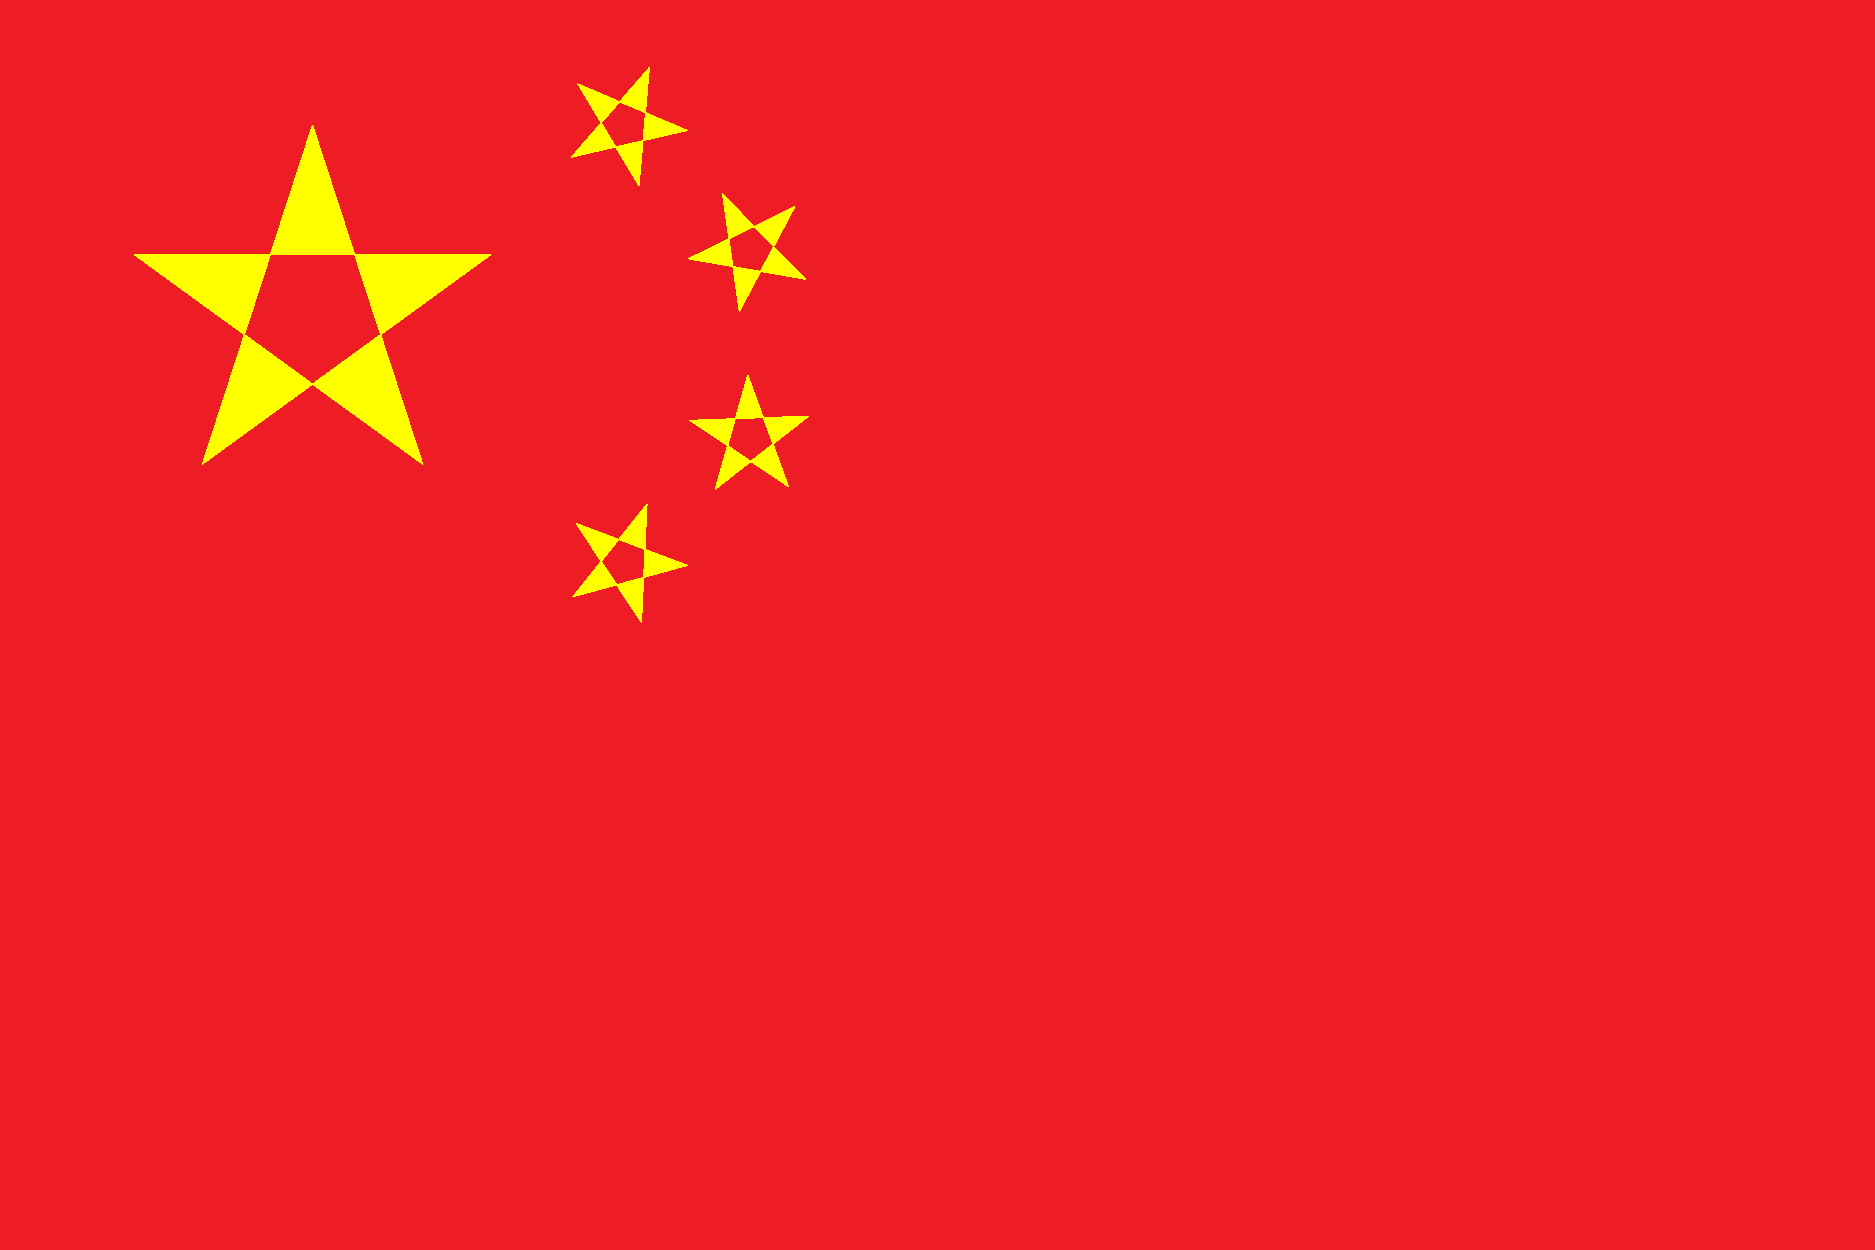
\includegraphics[width=1.0\linewidth]{Annexes/friseChronologique/img/Flag_of_the_People27s_Republic_of_China.pdf}
                \captionsetup{labelformat=empty}\refDrapeau{Drapeau the People27s Republic of China}{frise:Flag_of_the_People27s_Republic_of_China.pdf}
            \end{figure}
        \end{minipage}
    &
        \begin{minipage}{.65\textwidth}
            \textbf{-200} - \textbf{Invention du cerf-volant}
            
            Le cerf-volant est inventé en Chine vers 200 avant J.-C. Il sera utilisé pendant des siècles pour des applications militaires, religieuses et scientifiques. Au XVIIIe siècle, les cerfs-volants serviront aux premières expériences scientifiques sur l'aérodynamique.
            \begin{figure}[H]
                \legende{Cerf-volant moderne}{frise:Chinese_Kite.jpg}
            \end{figure}
        \end{minipage}
    &
        \begin{minipage}{.275\textwidth}
            \begin{figure}[H]
                \centering
                \includegraphics[width=1.0\linewidth]{Annexes/friseChronologique/img/Chinese_Kite.jpg}
            \end{figure}
        \end{minipage}
    \end{tabular}
\end{table}
\begin{table}[H]
    \centering
    \begin{tabular}{c l c}
        \begin{minipage}{.075\textwidth}
            \begin{figure}[H]
                \centering
                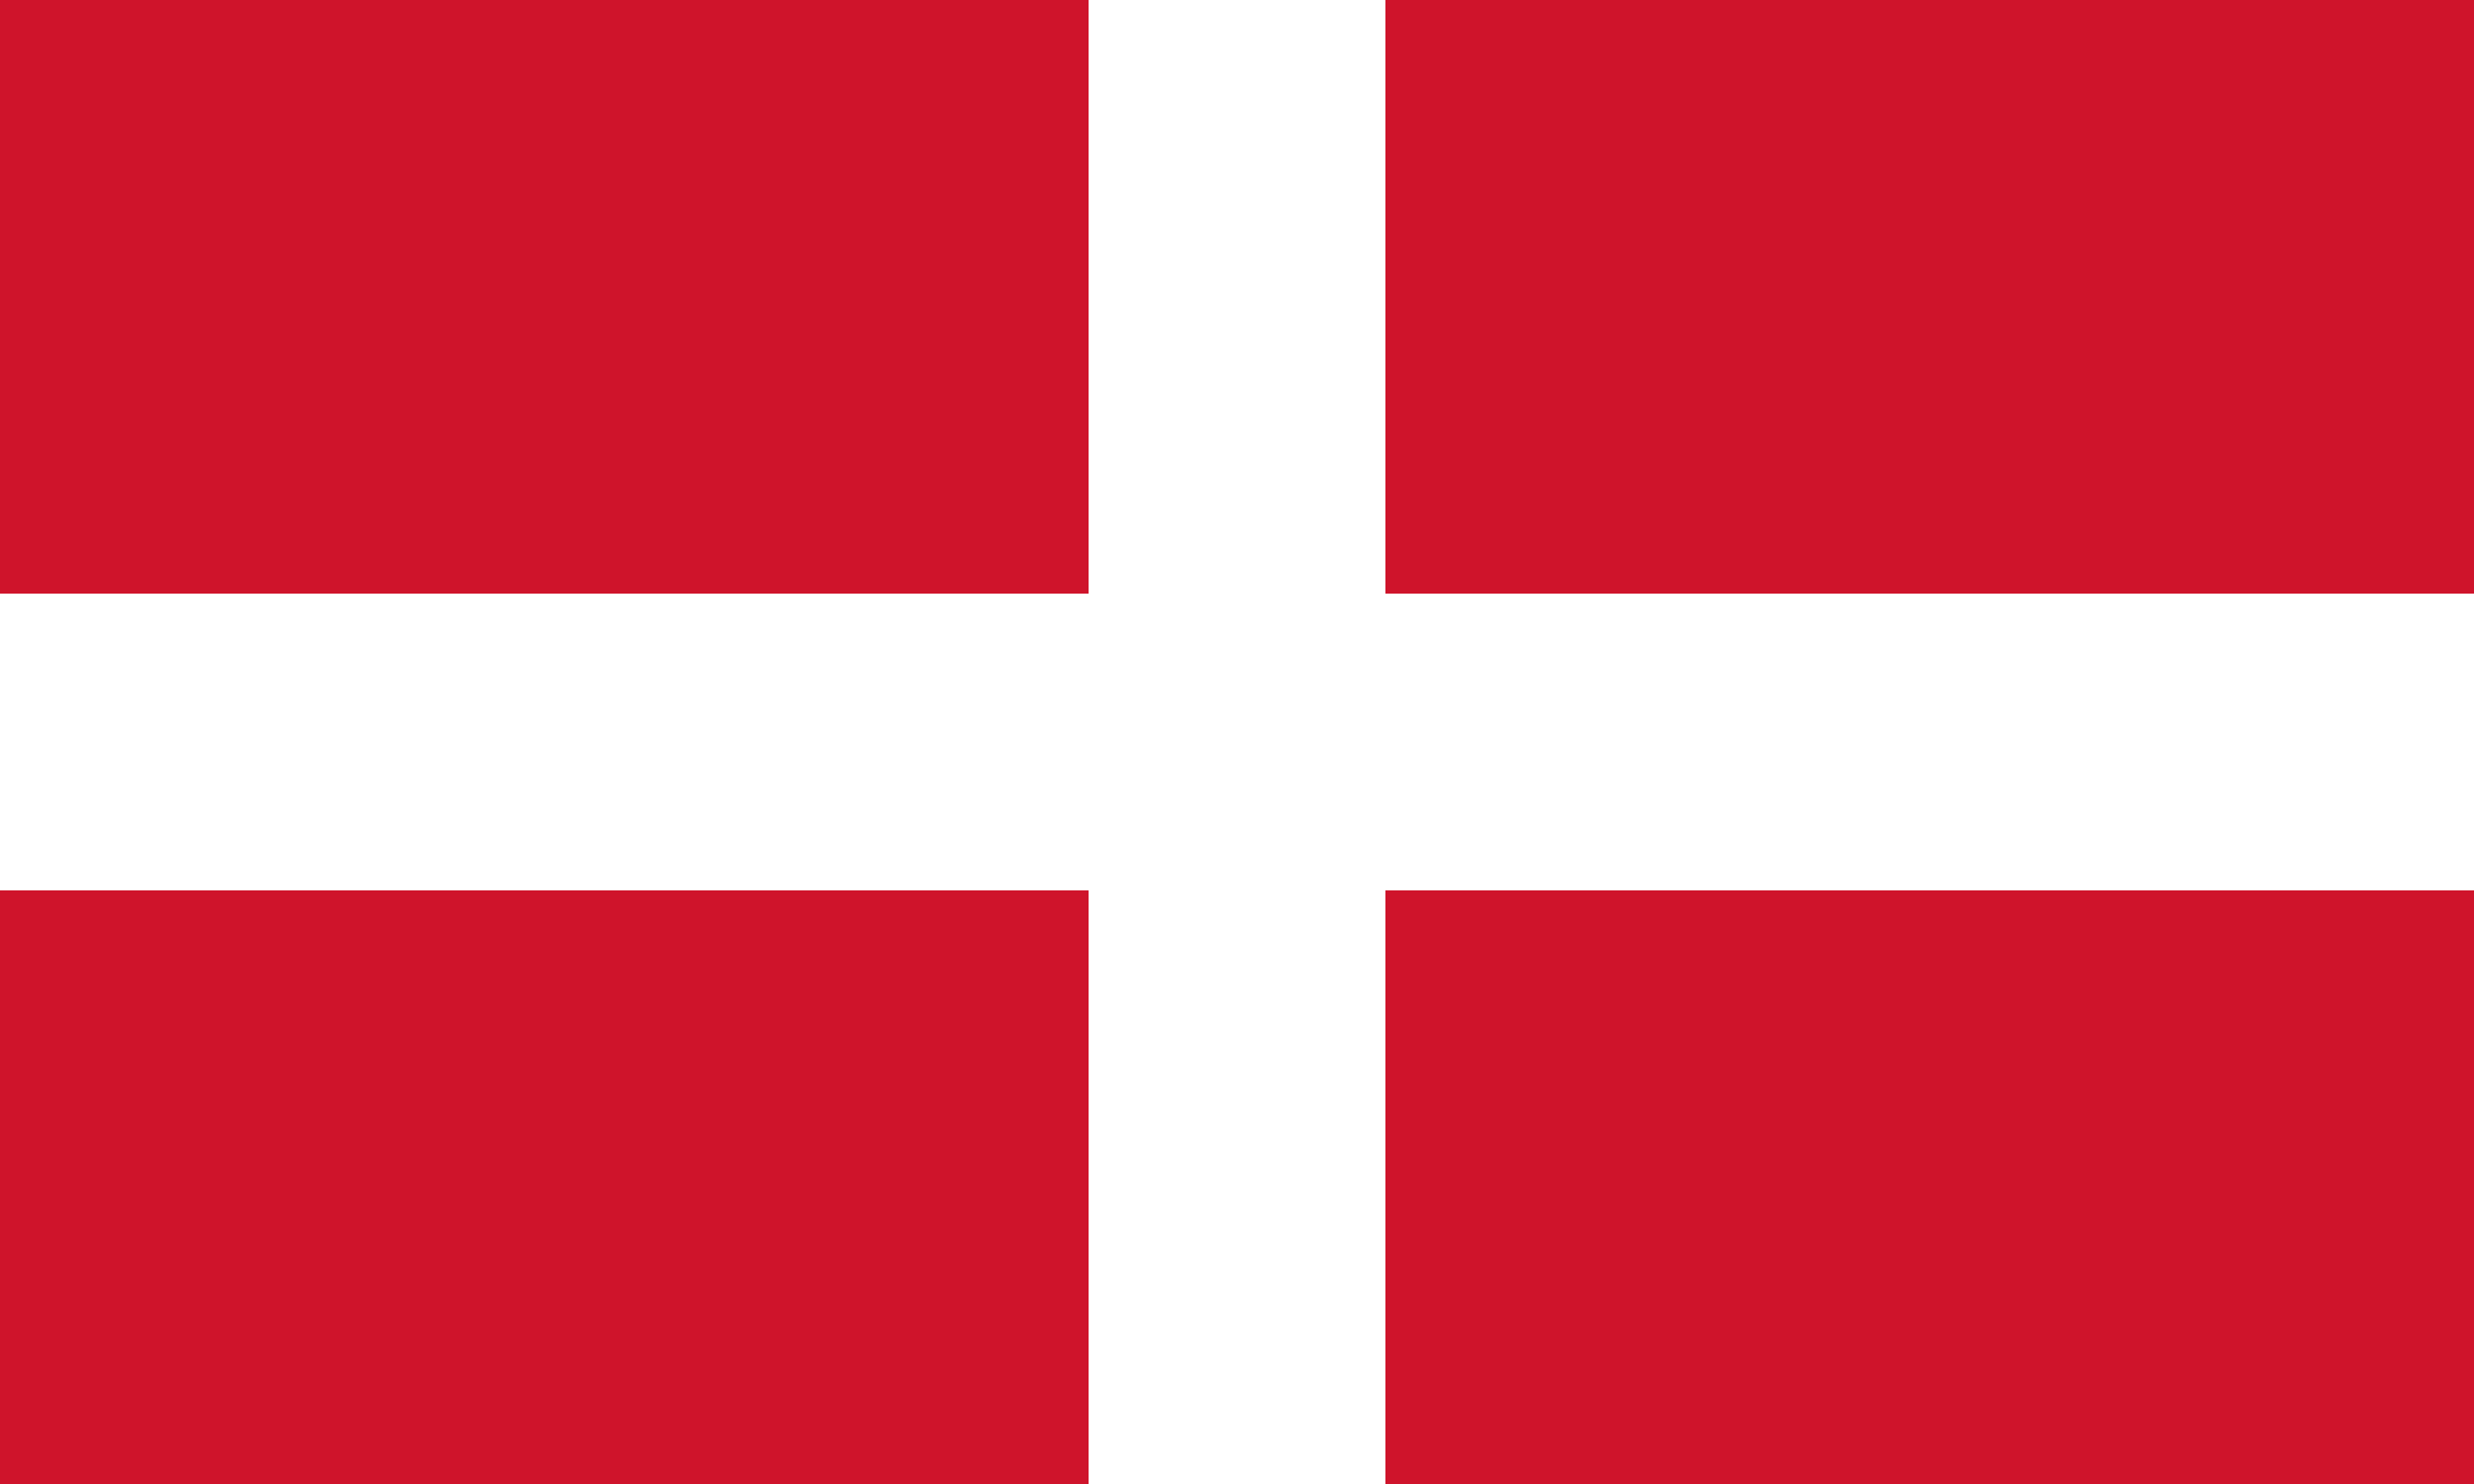
\includegraphics[width=1.0\linewidth]{Annexes/friseChronologique/img/Flag_of_John_the_Baptist.pdf}
                \captionsetup{labelformat=empty}\refDrapeau{Drapeau John the Baptist}{frise:Flag_of_John_the_Baptist.pdf}
            \end{figure}
        \end{minipage}
    &
        \begin{minipage}{.65\textwidth}
            \textbf{1485} - \textbf{Léonard de Vinci, visionnaire du vol}
            
            Léonard de Vinci étudie le vol des oiseaux et conçoit de nombreuses machines volantes dans ses carnets : l'ornithoptère (machine à ailes battantes), le parachute pyramidal, et une vis aérienne (ancêtre de l'hélicoptère). Bien que jamais construites de son vivant, ses études pionnières influenceront les inventeurs futurs.
            \begin{figure}[H]
                \legende{Étude de la vis aérienne de Léonard de Vinci}{frise:Leonardo_helicopter.JPG}
            \end{figure}
        \end{minipage}
    &
        \begin{minipage}{.275\textwidth}
            \begin{figure}[H]
                \centering
                \includegraphics[width=1.0\linewidth]{Annexes/friseChronologique/img/Leonardo_helicopter.JPG}
            \end{figure}
        \end{minipage}
    \end{tabular}
\end{table}
\section{L'aérostation}

\begin{table}[H]
    \centering
    \begin{tabular}{c l c}
        \begin{minipage}{.075\textwidth}
            \begin{figure}[H]
                \centering
                
\includegraphics[width=1.0\linewidth]{Annexes/friseChronologique/img/Flag_of_France.pdf}
                \captionsetup{labelformat=empty}\refDrapeau{Drapeau France}{frise:Flag_of_France.pdf}
            \end{figure}
            
            \centering\mdiBrevet
        \end{minipage}
    &
        \begin{minipage}{.65\textwidth}
            \textbf{1732} - \textbf{Henri Pitot invente le tube de Pitot}
            
            Le tube de Pitot est inventé en 1732 par le physicien Henri Pitot, pour la mesure de la vitesse des bateaux ou des vitesse d'écoulement de l'eau dans les rivière. Le tube de Pitot sera ensuite utilisé en aéronautique dans les dispositifs de mesure de vitesse des aéronefs.
            \begin{figure}[H]
                \legende{Portrait de Henri Pitot}{frise:Henri_de_Pitot.jpg}
            \end{figure}
        \end{minipage}
    &
        \begin{minipage}{.275\textwidth}
            \begin{figure}[H]
                \centering
                \includegraphics[width=1.0\linewidth]{Annexes/friseChronologique/img/Henri_de_Pitot.jpg}
            \end{figure}
        \end{minipage}
    \end{tabular}
\end{table}
\begin{table}[H]
    \centering
    \begin{tabular}{c l c}
        \begin{minipage}{.075\textwidth}
            \begin{figure}[H]
                \centering
                
\includegraphics[width=1.0\linewidth]{Annexes/friseChronologique/img/Flag_of_France.pdf}
                \captionsetup{labelformat=empty}\refDrapeau{Drapeau France}{frise:Flag_of_France.pdf}
            \end{figure}
            
            \centering\mdiAirBalloon
        \end{minipage}
    &
        \begin{minipage}{.65\textwidth}
            \textbf{1783} - \textbf{Premier vol en montgolfière}
            
            Pilâtre de Rosier s'élève dans le ciel grâce à la montgolfière des frères Montgoflier
            \begin{figure}[H]
                \legende{Ascension captive d'une montgolfière (Jean-François Pilâtre de Rozier) dans les jardins de la papèterie Réveillon, le 19 octobre 1783.}{frise:Montgolfiere_1783.jpg}
            \end{figure}
        \end{minipage}
    &
        \begin{minipage}{.275\textwidth}
            \begin{figure}[H]
                \centering
                \includegraphics[width=1.0\linewidth]{Annexes/friseChronologique/img/Montgolfiere_1783.jpg}
            \end{figure}
        \end{minipage}
    \end{tabular}
\end{table}
\begin{table}[H]
    \centering
    \begin{tabular}{c l c}
        \begin{minipage}{.075\textwidth}
            \begin{figure}[H]
                \centering
                
\includegraphics[width=1.0\linewidth]{Annexes/friseChronologique/img/Flag_of_France.pdf}
                \captionsetup{labelformat=empty}\refDrapeau{Drapeau France}{frise:Flag_of_France.pdf}
            \end{figure}
            
            \centering\mdiAirBalloon
        \end{minipage}
    &
        \begin{minipage}{.65\textwidth}
            \textbf{1785} - \textbf{Première traversée de la manche}
            
            Jean-Pierre Blanchard traverse la Manche en ballon
            \begin{figure}[H]
                \legende{Traversée en ballon du Pas-de-Calais par Blanchard et Jefferies (1785)}{frise:Early_flight_02562u_28729.jpg}
            \end{figure}
        \end{minipage}
    &
        \begin{minipage}{.275\textwidth}
            \begin{figure}[H]
                \centering
                \includegraphics[width=1.0\linewidth]{Annexes/friseChronologique/img/Early_flight_02562u_28729.jpg}
            \end{figure}
        \end{minipage}
    \end{tabular}
\end{table}
\begin{table}[H]
    \centering
    \begin{tabular}{c l c}
        \begin{minipage}{.075\textwidth}
            \begin{figure}[H]
                \centering
                
\includegraphics[width=1.0\linewidth]{Annexes/friseChronologique/img/Flag_of_France.pdf}
                \captionsetup{labelformat=empty}\refDrapeau{Drapeau France}{frise:Flag_of_France.pdf}
            \end{figure}
            
            \centering\mdiAirBalloon
            
            \centering\mdiParachute
        \end{minipage}
    &
        \begin{minipage}{.65\textwidth}
            \textbf{1797} - \textbf{Premier saut en parachute}
            
            André-Jacques Garnerin effectue le premier saut en parachute, depuis un ballon
            \begin{figure}[H]
                \legende{N°. 4 – Descente de Jacques Garnerin en parachute (1797)}{frise:Early_flight_02561u_28429.jpg}
            \end{figure}
        \end{minipage}
    &
        \begin{minipage}{.275\textwidth}
            \begin{figure}[H]
                \centering
                \includegraphics[width=1.0\linewidth]{Annexes/friseChronologique/img/Early_flight_02561u_28429.jpg}
            \end{figure}
        \end{minipage}
    \end{tabular}
\end{table}
\begin{table}[H]
    \centering
    \begin{tabular}{c l c}
        \begin{minipage}{.075\textwidth}
            \begin{figure}[H]
                \centering
                
\includegraphics[width=1.0\linewidth]{Annexes/friseChronologique/img/Flag_of_France.pdf}
                \captionsetup{labelformat=empty}\refDrapeau{Drapeau France}{frise:Flag_of_France.pdf}
            \end{figure}
            
            \centering\mdiAirBalloon
        \end{minipage}
    &
        \begin{minipage}{.65\textwidth}
            \textbf{1852} - \textbf{Premier vol en dirigeable}
            
            L'ingénieur français Henri Giffard fit voler le premier dirigeable
        \end{minipage}
    &
        \begin{minipage}{.275\textwidth}
            \begin{figure}[H]
                \centering
                \includegraphics[width=1.0\linewidth]{Annexes/friseChronologique/vide.pdf}
            \end{figure}
        \end{minipage}
    \end{tabular}
\end{table}
\begin{table}[H]
    \centering
    \begin{tabular}{c l c}
        \begin{minipage}{.075\textwidth}
            \begin{figure}[H]
                \centering
                
\includegraphics[width=1.0\linewidth]{Annexes/friseChronologique/img/Flag_of_France.pdf}
                \captionsetup{labelformat=empty}\refDrapeau{Drapeau France}{frise:Flag_of_France.pdf}
            \end{figure}
            
            \centering\mdiAirBalloon
        \end{minipage}
    &
        \begin{minipage}{.65\textwidth}
            \textbf{1858} - \textbf{Nadar réalise la première photographie aérienne}
            
            Felix Tournachon dit "Nadar" devient le premier photographe aérien en réalisant une prise de vue de Paris depuis un ballon.
            \begin{figure}[H]
                \legende{Nadar élevant la Photographie à la hauteur de l'Art., lithographie d'Honoré Daumier parue dans Le Boulevard, le 25 mai 1863}{frise:HonorC3A9_Daumier2C_Nadar_C3A9levant_la_Photographie_C3A0_la_hauteur_de_l27Art2C_18622C_NGA_42966.jpg}
            \end{figure}
        \end{minipage}
    &
        \begin{minipage}{.275\textwidth}
            \begin{figure}[H]
                \centering
                \includegraphics[width=1.0\linewidth]{Annexes/friseChronologique/img/HonorC3A9_Daumier2C_Nadar_C3A9levant_la_Photographie_C3A0_la_hauteur_de_l27Art2C_18622C_NGA_42966.jpg}
            \end{figure}
        \end{minipage}
    \end{tabular}
\end{table}
\section{Les pionniers du plus lourd que l'air}

\begin{table}[H]
    \centering
    \begin{tabular}{c l c}
        \begin{minipage}{.075\textwidth}
            \begin{figure}[H]
                \centering
                
\includegraphics[width=1.0\linewidth]{Annexes/friseChronologique/img/Flag_of_France.pdf}
                \captionsetup{labelformat=empty}\refDrapeau{Drapeau France}{frise:Flag_of_France.pdf}
            \end{figure}
        \end{minipage}
    &
        \begin{minipage}{.65\textwidth}
            \textbf{1890} - \textbf{Clément Ader met au point l'Eole}
            
            Clément Ader, ingénieur français, conçoit l'Eole puis les Avions, aérodynes en forme de chauves-souris. Bien que Clément Ader affirma à partir de 1906 que ses aérodynes soient parvnus à réaliser des vols de 300 m, on manque de preuve pour attester ces affirmations. Pour cette raison, on ne retient pas Ader comme ayant été le premier à effectuer un vol contrôlé.
            \begin{figure}[H]
                \legende{L’Avion III de Clément Ader}{frise:Avion_III_Art_et_Metiers.jpg}
            \end{figure}
        \end{minipage}
    &
        \begin{minipage}{.275\textwidth}
            \begin{figure}[H]
                \centering
                \includegraphics[width=1.0\linewidth]{Annexes/friseChronologique/img/Avion_III_Art_et_Metiers.jpg}
            \end{figure}
        \end{minipage}
    \end{tabular}
\end{table}
\begin{table}[H]
    \centering
    \begin{tabular}{c l c}
        \begin{minipage}{.075\textwidth}
            \begin{figure}[H]
                \centering
                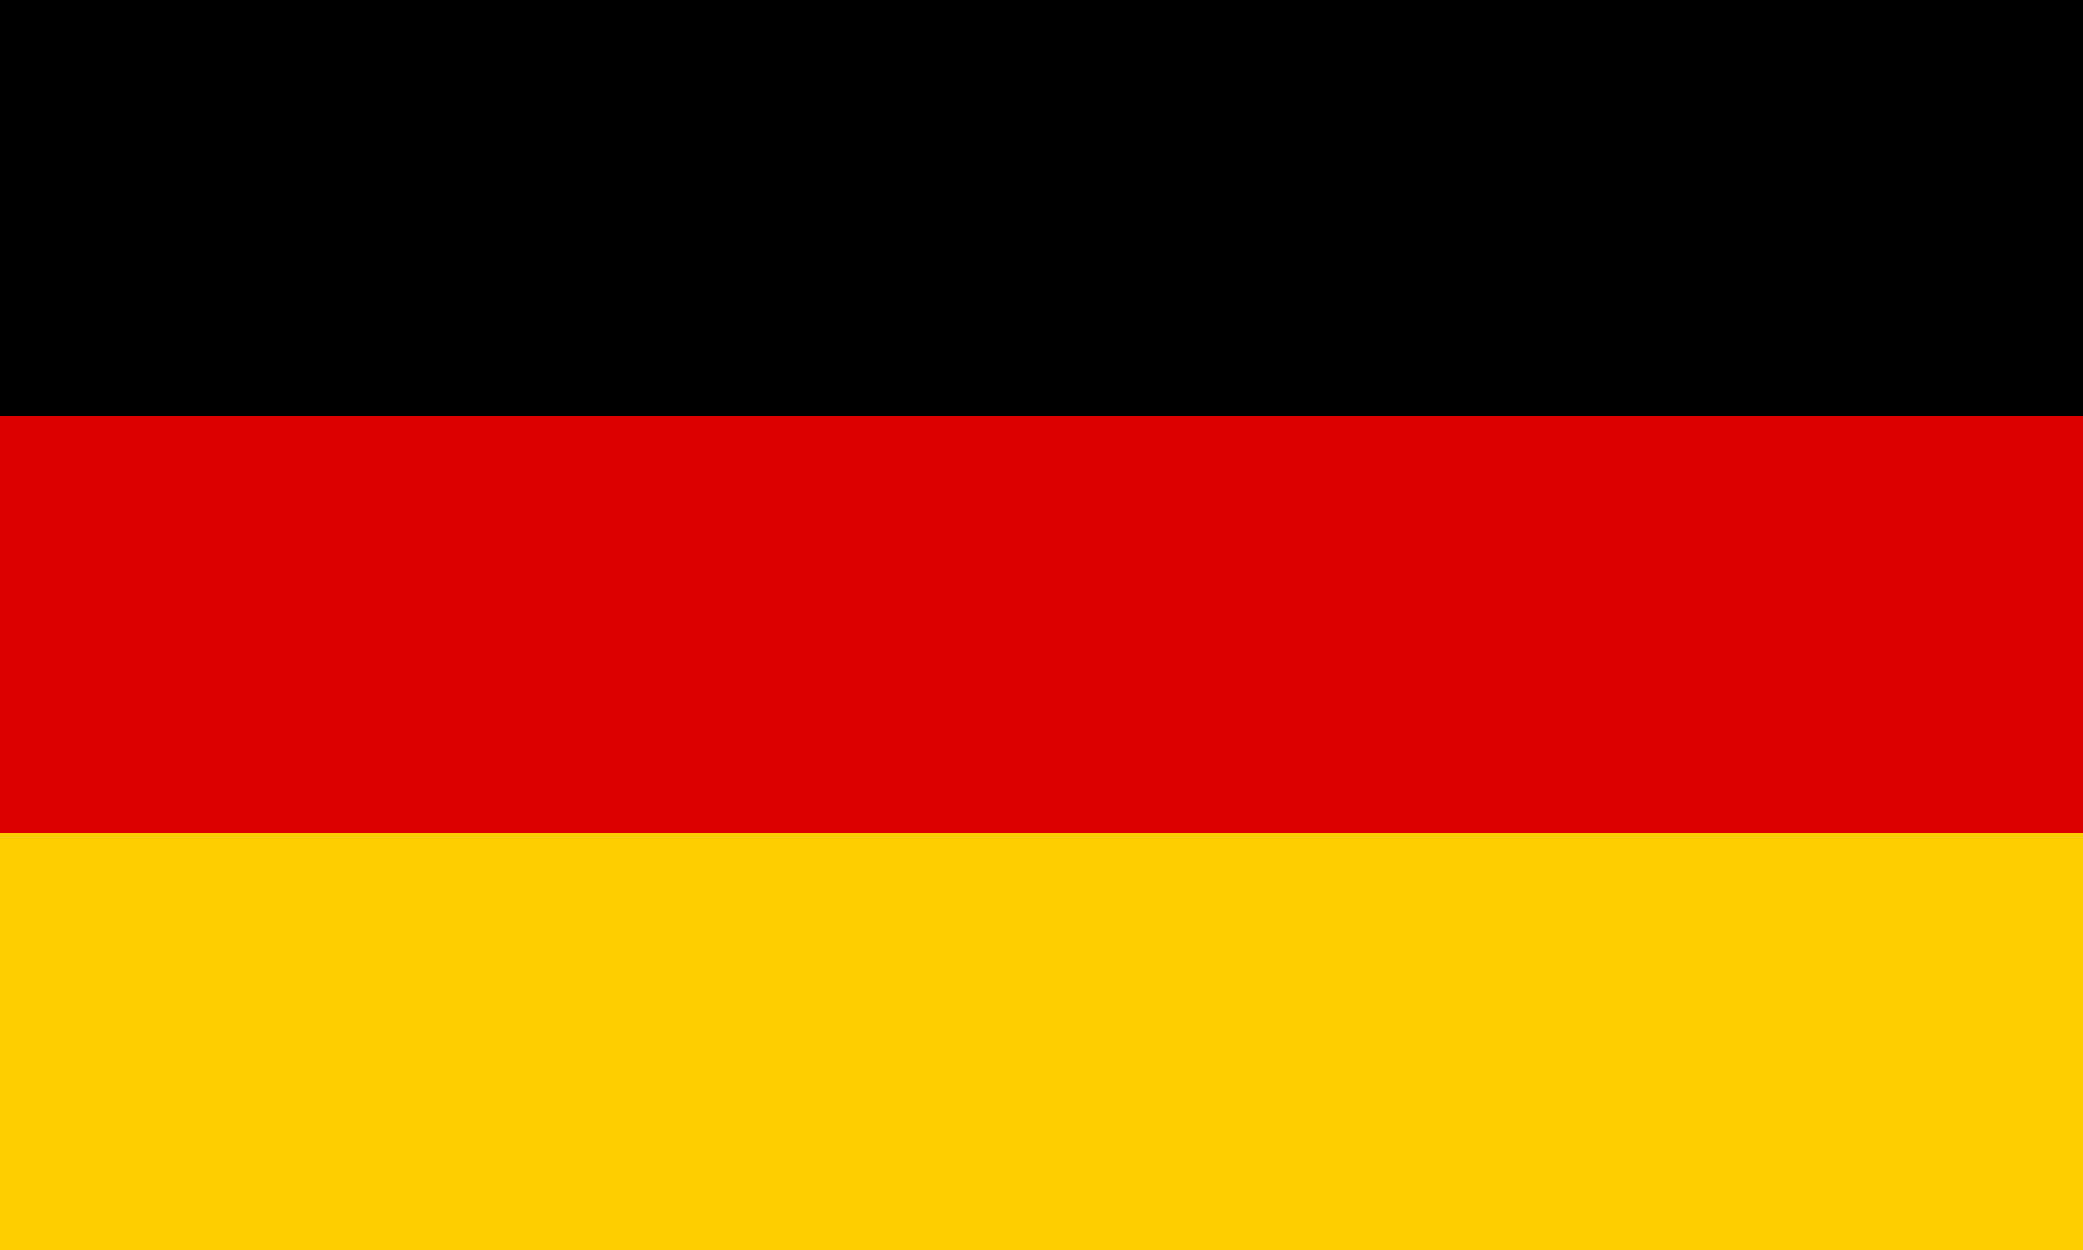
\includegraphics[width=1.0\linewidth]{Annexes/friseChronologique/img/Flag_of_Germany.pdf}
                \captionsetup{labelformat=empty}\refDrapeau{Drapeau Germany}{frise:Flag_of_Germany.pdf}
            \end{figure}
        \end{minipage}
    &
        \begin{minipage}{.65\textwidth}
            \textbf{1891} - \textbf{Premier vol en planeur}
            
            L'ingénieur allemand Otto Lilienthal fait voler son planeur, en se lancant depuis une colline
            \begin{figure}[H]
                \legende{L'un des vols d'Otto Lilienthal, ici en 1895}{frise:Otto_Lilienthal_gliding_experiment_ppmsca.02546.jpg}
            \end{figure}
        \end{minipage}
    &
        \begin{minipage}{.275\textwidth}
            \begin{figure}[H]
                \centering
                \includegraphics[width=1.0\linewidth]{Annexes/friseChronologique/img/Otto_Lilienthal_gliding_experiment_ppmsca.02546.jpg}
            \end{figure}
        \end{minipage}
    \end{tabular}
\end{table}
\begin{table}[H]
    \centering
    \begin{tabular}{c l c}
        \begin{minipage}{.075\textwidth}
            \begin{figure}[H]
                \centering
                
\includegraphics[width=1.0\linewidth]{Annexes/friseChronologique/img/Flag_of_the_United_States_28DDD-F-416E_specifications29.pdf}
                \captionsetup{labelformat=empty}\refDrapeau{Drapeau the United States 28DDD-F-416E specifications29}{frise:Flag_of_the_United_States_28DDD-F-416E_specifications29.pdf}
            \end{figure}
        \end{minipage}
    &
        \begin{minipage}{.65\textwidth}
            \textbf{1896} - \textbf{Octave Chanute et le vol plané}
            
            L'ingénieur franco-américain Octave Chanute perfectionne les planeurs et effectue des centaines de vols. Ses travaux, notamment sur la structure biplan, influenceront directement les frères Wright. Il joue un rôle crucial dans la diffusion des connaissances aéronautiques.
            \begin{figure}[H]
                \legende{Planeur d'Octave Chanute en 1896}{frise:Chanute-Herring_1896_hang_glider.jpg}
            \end{figure}
        \end{minipage}
    &
        \begin{minipage}{.275\textwidth}
            \begin{figure}[H]
                \centering
                \includegraphics[width=1.0\linewidth]{Annexes/friseChronologique/img/Chanute-Herring_1896_hang_glider.jpg}
            \end{figure}
        \end{minipage}
    \end{tabular}
\end{table}
\begin{table}[H]
    \centering
    \begin{tabular}{c l c}
        \begin{minipage}{.075\textwidth}
            \begin{figure}[H]
                \centering
                
\includegraphics[width=1.0\linewidth]{Annexes/friseChronologique/img/Flag_of_France.pdf}
                \captionsetup{labelformat=empty}\refDrapeau{Drapeau France}{frise:Flag_of_France.pdf}
            \end{figure}
        \end{minipage}
    &
        \begin{minipage}{.65\textwidth}
            \textbf{19 octobre 1901} - \textbf{Alberto Santos Dumont contourne la Tour Eiffel en dirigeable}
            
            
            \begin{figure}[H]
                \legende{Internet Archive Book Images}{frise:Santos-Dumont_flight_around_the_Eiffel_Tower.jpg}
            \end{figure}
        \end{minipage}
    &
        \begin{minipage}{.275\textwidth}
            \begin{figure}[H]
                \centering
                \includegraphics[width=1.0\linewidth]{Annexes/friseChronologique/img/Santos-Dumont_flight_around_the_Eiffel_Tower.jpg}
            \end{figure}
        \end{minipage}
    \end{tabular}
\end{table}
\begin{table}[H]
    \centering
    \begin{tabular}{c l c}
        \begin{minipage}{.075\textwidth}
            \begin{figure}[H]
                \centering
                
\includegraphics[width=1.0\linewidth]{Annexes/friseChronologique/img/Flag_of_the_United_States_28DDD-F-416E_specifications29.pdf}
                \captionsetup{labelformat=empty}\refDrapeau{Drapeau the United States 28DDD-F-416E specifications29}{frise:Flag_of_the_United_States_28DDD-F-416E_specifications29.pdf}
            \end{figure}
        \end{minipage}
    &
        \begin{minipage}{.65\textwidth}
            \textbf{1903} - \textbf{Premier vol d'un avion}
            
            Les frères Orville et Wilbur Wright font voler leur avion aux Etats-Unis.
Il s'agit du premier vol contrôlé d'un aérodyne motorisé
            \begin{figure}[H]
                \legende{Premier vol motorisé des frères Wright le 17 décembre 1903 sur Flyer.}{frise:Wrightflyer.jpg}
            \end{figure}
        \end{minipage}
    &
        \begin{minipage}{.275\textwidth}
            \begin{figure}[H]
                \centering
                \includegraphics[width=1.0\linewidth]{Annexes/friseChronologique/img/Wrightflyer.jpg}
            \end{figure}
        \end{minipage}
    \end{tabular}
\end{table}
\begin{table}[H]
    \centering
    \begin{tabular}{c l c}
        \begin{minipage}{.075\textwidth}
            \begin{figure}[H]
                \centering
                
\includegraphics[width=1.0\linewidth]{Annexes/friseChronologique/img/Flag_of_France.pdf}
                \captionsetup{labelformat=empty}\refDrapeau{Drapeau France}{frise:Flag_of_France.pdf}
            \end{figure}
            
            \centering\mdiBrevet
        \end{minipage}
    &
        \begin{minipage}{.65\textwidth}
            \textbf{22 janvier 1907} - \textbf{Invention du manche à balai}
            
            Robert Esnault-Pelterie dépose le brevet pour le manche à balai, permettant de diriger les aéronefs
            \begin{figure}[H]
                \legende{Portrait de Robert Esnault-Pelterie}{frise:Robert_Esnault-Pelterie_1909.jpg}
            \end{figure}
        \end{minipage}
    &
        \begin{minipage}{.275\textwidth}
            \begin{figure}[H]
                \centering
                \includegraphics[width=1.0\linewidth]{Annexes/friseChronologique/img/Robert_Esnault-Pelterie_1909.jpg}
            \end{figure}
        \end{minipage}
    \end{tabular}
\end{table}
\begin{table}[H]
    \centering
    \begin{tabular}{c l c}
        \begin{minipage}{.075\textwidth}
            \begin{figure}[H]
                \centering
                
\includegraphics[width=1.0\linewidth]{Annexes/friseChronologique/img/Flag_of_France.pdf}
                \captionsetup{labelformat=empty}\refDrapeau{Drapeau France}{frise:Flag_of_France.pdf}
            \end{figure}
            
            \centering\mdiFemale
        \end{minipage}
    &
        \begin{minipage}{.65\textwidth}
            \textbf{08 juillet 1908} - \textbf{Thérèse Peltier, première femme à quitter le sol}
            
            Le 8 juillet 1908, Thérèse Peltier devient la premier femme à quitter le sol avec un aéronef, dans un avion piloté par son compagnon Léon Delagrange.

Elle deviendra la première femme à voler seule à bord d'un avion quelque mois plus tard, lors de son lâcher solo.
            \begin{figure}[H]
                \legende{Thérèse Peltier à Issy-les-Moulineaux le 17 September 1908}{frise:ThC3A9rC3A8se_Peltier_1908.jpg}
            \end{figure}
        \end{minipage}
    &
        \begin{minipage}{.275\textwidth}
            \begin{figure}[H]
                \centering
                \includegraphics[width=1.0\linewidth]{Annexes/friseChronologique/img/ThC3A9rC3A8se_Peltier_1908.jpg}
            \end{figure}
        \end{minipage}
    \end{tabular}
\end{table}
\begin{table}[H]
    \centering
    \begin{tabular}{c l c}
        \begin{minipage}{.075\textwidth}
            \begin{figure}[H]
                \centering
                
\includegraphics[width=1.0\linewidth]{Annexes/friseChronologique/img/Flag_of_France.pdf}
                \captionsetup{labelformat=empty}\refDrapeau{Drapeau France}{frise:Flag_of_France.pdf}
            \end{figure}
        \end{minipage}
    &
        \begin{minipage}{.65\textwidth}
            \textbf{25 juillet 1909} - \textbf{Louis Blériot traverse la manche}
            
            "L'Angleterre n'est plus une île !" Le 25 juillet 1909, Louis Blériot relie Calais à Douvres à bord de son  Blériot XI.
            \begin{figure}[H]
                \legende{Blériot aux commandes de l'appareil de la traversée à la fête de Port-Aviation, le 4 juillet 1909.}{frise:Btv1b8433368f-p044_BlC3A9riot_C3A0_la_fC3AAte_de_Port-Aviation2C_dimanche_4_juillet_1909.jpg}
            \end{figure}
        \end{minipage}
    &
        \begin{minipage}{.275\textwidth}
            \begin{figure}[H]
                \centering
                \includegraphics[width=1.0\linewidth]{Annexes/friseChronologique/img/Btv1b8433368f-p044_BlC3A9riot_C3A0_la_fC3AAte_de_Port-Aviation2C_dimanche_4_juillet_1909.jpg}
            \end{figure}
        \end{minipage}
    \end{tabular}
\end{table}
\begin{table}[H]
    \centering
    \begin{tabular}{c l c}
        \begin{minipage}{.075\textwidth}
            \begin{figure}[H]
                \centering
                
\includegraphics[width=1.0\linewidth]{Annexes/friseChronologique/img/Flag_of_France.pdf}
                \captionsetup{labelformat=empty}\refDrapeau{Drapeau France}{frise:Flag_of_France.pdf}
            \end{figure}
        \end{minipage}
    &
        \begin{minipage}{.65\textwidth}
            \textbf{07 octobre 1909} - \textbf{Louis Blériot obtient le premier brevet de pilote}
            
            Le brevet de pilote n°1 est délivré à Louis Blériot

Le 7 octobre 1909, l'Aéro-Club de France décide de décerner un brevet de pilote à seize pionniers de l'aviation. Personne n’osant faire passer un examen à ces pionniers, un comité prit la liste des pilotes et les classa par ordre alphabétique. Son nom commençant par un B, Louis Blériot se voit attribuer le brevet de pilote numéro 1. L’instauration du brevet de pilote intervient le 1er janvier 1910.
            \begin{figure}[H]
                \legende{Avant de délivrer des brevets de pilotes d'avion, l'Aéroclub de France délivrait également des brevets aux pilotes de ballons. Brevet de pilote aéronaute décerné par l'Aéro-Club de France à Paul Tissandier (1904).}{frise:Brevet_de_pilote_aC3A9ronaute_1904.jpg}
            \end{figure}
        \end{minipage}
    &
        \begin{minipage}{.275\textwidth}
            \begin{figure}[H]
                \centering
                \includegraphics[width=1.0\linewidth]{Annexes/friseChronologique/img/Brevet_de_pilote_aC3A9ronaute_1904.jpg}
            \end{figure}
        \end{minipage}
    \end{tabular}
\end{table}
\begin{table}[H]
    \centering
    \begin{tabular}{c l c}
        \begin{minipage}{.075\textwidth}
            \begin{figure}[H]
                \centering
                
\includegraphics[width=1.0\linewidth]{Annexes/friseChronologique/img/Flag_of_France.pdf}
                \captionsetup{labelformat=empty}\refDrapeau{Drapeau France}{frise:Flag_of_France.pdf}
            \end{figure}
            
            \centering\mdiFemale
        \end{minipage}
    &
        \begin{minipage}{.65\textwidth}
            \textbf{08 mars 1910} - \textbf{Élisa Deroche, première femme brevetée pilote}
            
            Élisa Deroche s'interesse à l'aviation depuis l'année 1906.
Fin 1909, elle effectue son premier vol solo, et son brevet (le n°36) lui sera délivré quelques mois plus tard, le 8 mars 1910.

La semaine internationale des femmes de l'air marque désormais chaque année cette date historique, puisque cette semaine est positionnée sur la semaine du 8 mars. 

            \begin{figure}[H]
                \legende{Elise Deroche aux commandes d'un biplan Voisin.}{frise:Les_Maitres_de_l27aviation._Mme._la_Baronne_de_Laroche2C_aviatrice2C_au_poste_de_direction_d27un_biplan_Voisin._cph.3c07402.jpg}
            \end{figure}
        \end{minipage}
    &
        \begin{minipage}{.275\textwidth}
            \begin{figure}[H]
                \centering
                \includegraphics[width=1.0\linewidth]{Annexes/friseChronologique/img/Les_Maitres_de_l27aviation._Mme._la_Baronne_de_Laroche2C_aviatrice2C_au_poste_de_direction_d27un_biplan_Voisin._cph.3c07402.jpg}
            \end{figure}
        \end{minipage}
    \end{tabular}
\end{table}
\begin{table}[H]
    \centering
    \begin{tabular}{c l c}
        \begin{minipage}{.075\textwidth}
            \begin{figure}[H]
                \centering
                
\includegraphics[width=1.0\linewidth]{Annexes/friseChronologique/img/Flag_of_France.pdf}
                \captionsetup{labelformat=empty}\refDrapeau{Drapeau France}{frise:Flag_of_France.pdf}
            \end{figure}
        \end{minipage}
    &
        \begin{minipage}{.65\textwidth}
            \textbf{28 mars 1910} - \textbf{Premier vol d'un hydravion}
            
            L'ingénieur français Henri Fabre devient le premier à décoller d'un plan d'eau avec un aéronef qui dispose de son propre moyen de propulsion. Cette date marque l'entrée dans l'ère de l'hydraviation qui aura son âge d'or sur la période de l'entre 2 guerres.
            \begin{figure}[H]
                \legende{Hydroplane d'Henri Fabre}{frise:Hydroplane_28de_Henri29_Fabre_28Monaco2C_concours_de_canots_automobiles2C_2_-17_avril29_1911_-_btv1b53240713d.jpg}
            \end{figure}
        \end{minipage}
    &
        \begin{minipage}{.275\textwidth}
            \begin{figure}[H]
                \centering
                \includegraphics[width=1.0\linewidth]{Annexes/friseChronologique/img/Hydroplane_28de_Henri29_Fabre_28Monaco2C_concours_de_canots_automobiles2C_2_-17_avril29_1911_-_btv1b53240713d.jpg}
            \end{figure}
        \end{minipage}
    \end{tabular}
\end{table}
\begin{table}[H]
    \centering
    \begin{tabular}{c l c}
        \begin{minipage}{.075\textwidth}
            \begin{figure}[H]
                \centering
                
\includegraphics[width=1.0\linewidth]{Annexes/friseChronologique/img/Flag_of_France.pdf}
                \captionsetup{labelformat=empty}\refDrapeau{Drapeau France}{frise:Flag_of_France.pdf}
            \end{figure}
            
            \centering\mdiBrevet
        \end{minipage}
    &
        \begin{minipage}{.65\textwidth}
            \textbf{1911} - \textbf{Raoul Badin invente l'anémomètre}
            
            L'inventeur français invente un dispositif permettant la mesure de la vitesse de l'air dans lequel évolue un aéronef. L'anémomère est parfois appelé "badin" du nom de cet inventeur
            \begin{figure}[H]
                \legende{Illustration d'un anémomètre moderne}{frise:Airspeed_indicator.pdf}
            \end{figure}
        \end{minipage}
    &
        \begin{minipage}{.275\textwidth}
            \begin{figure}[H]
                \centering
                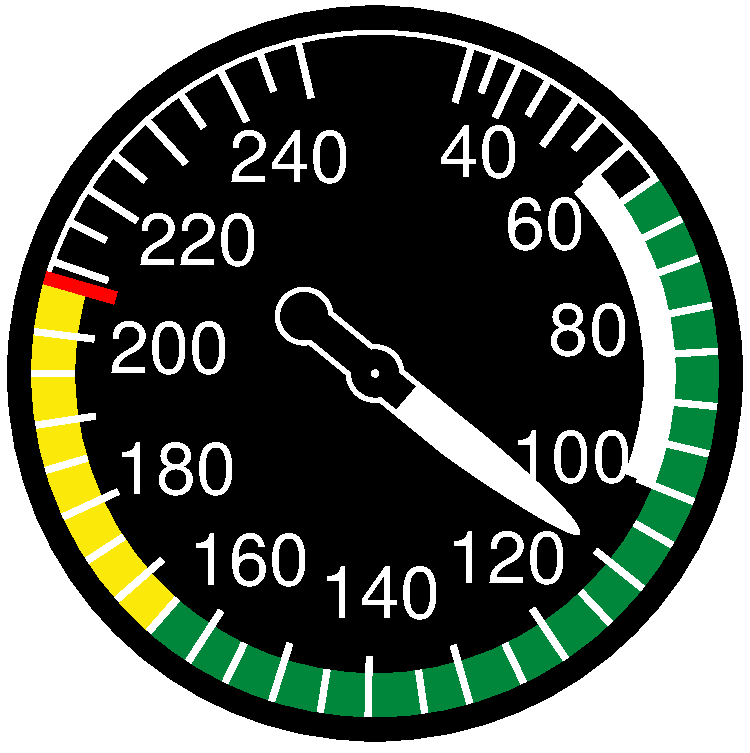
\includegraphics[width=1.0\linewidth]{Annexes/friseChronologique/img/Airspeed_indicator.pdf}
            \end{figure}
        \end{minipage}
    \end{tabular}
\end{table}
\begin{table}[H]
    \centering
    \begin{tabular}{c l c}
        \begin{minipage}{.075\textwidth}
            \begin{figure}[H]
                \centering
                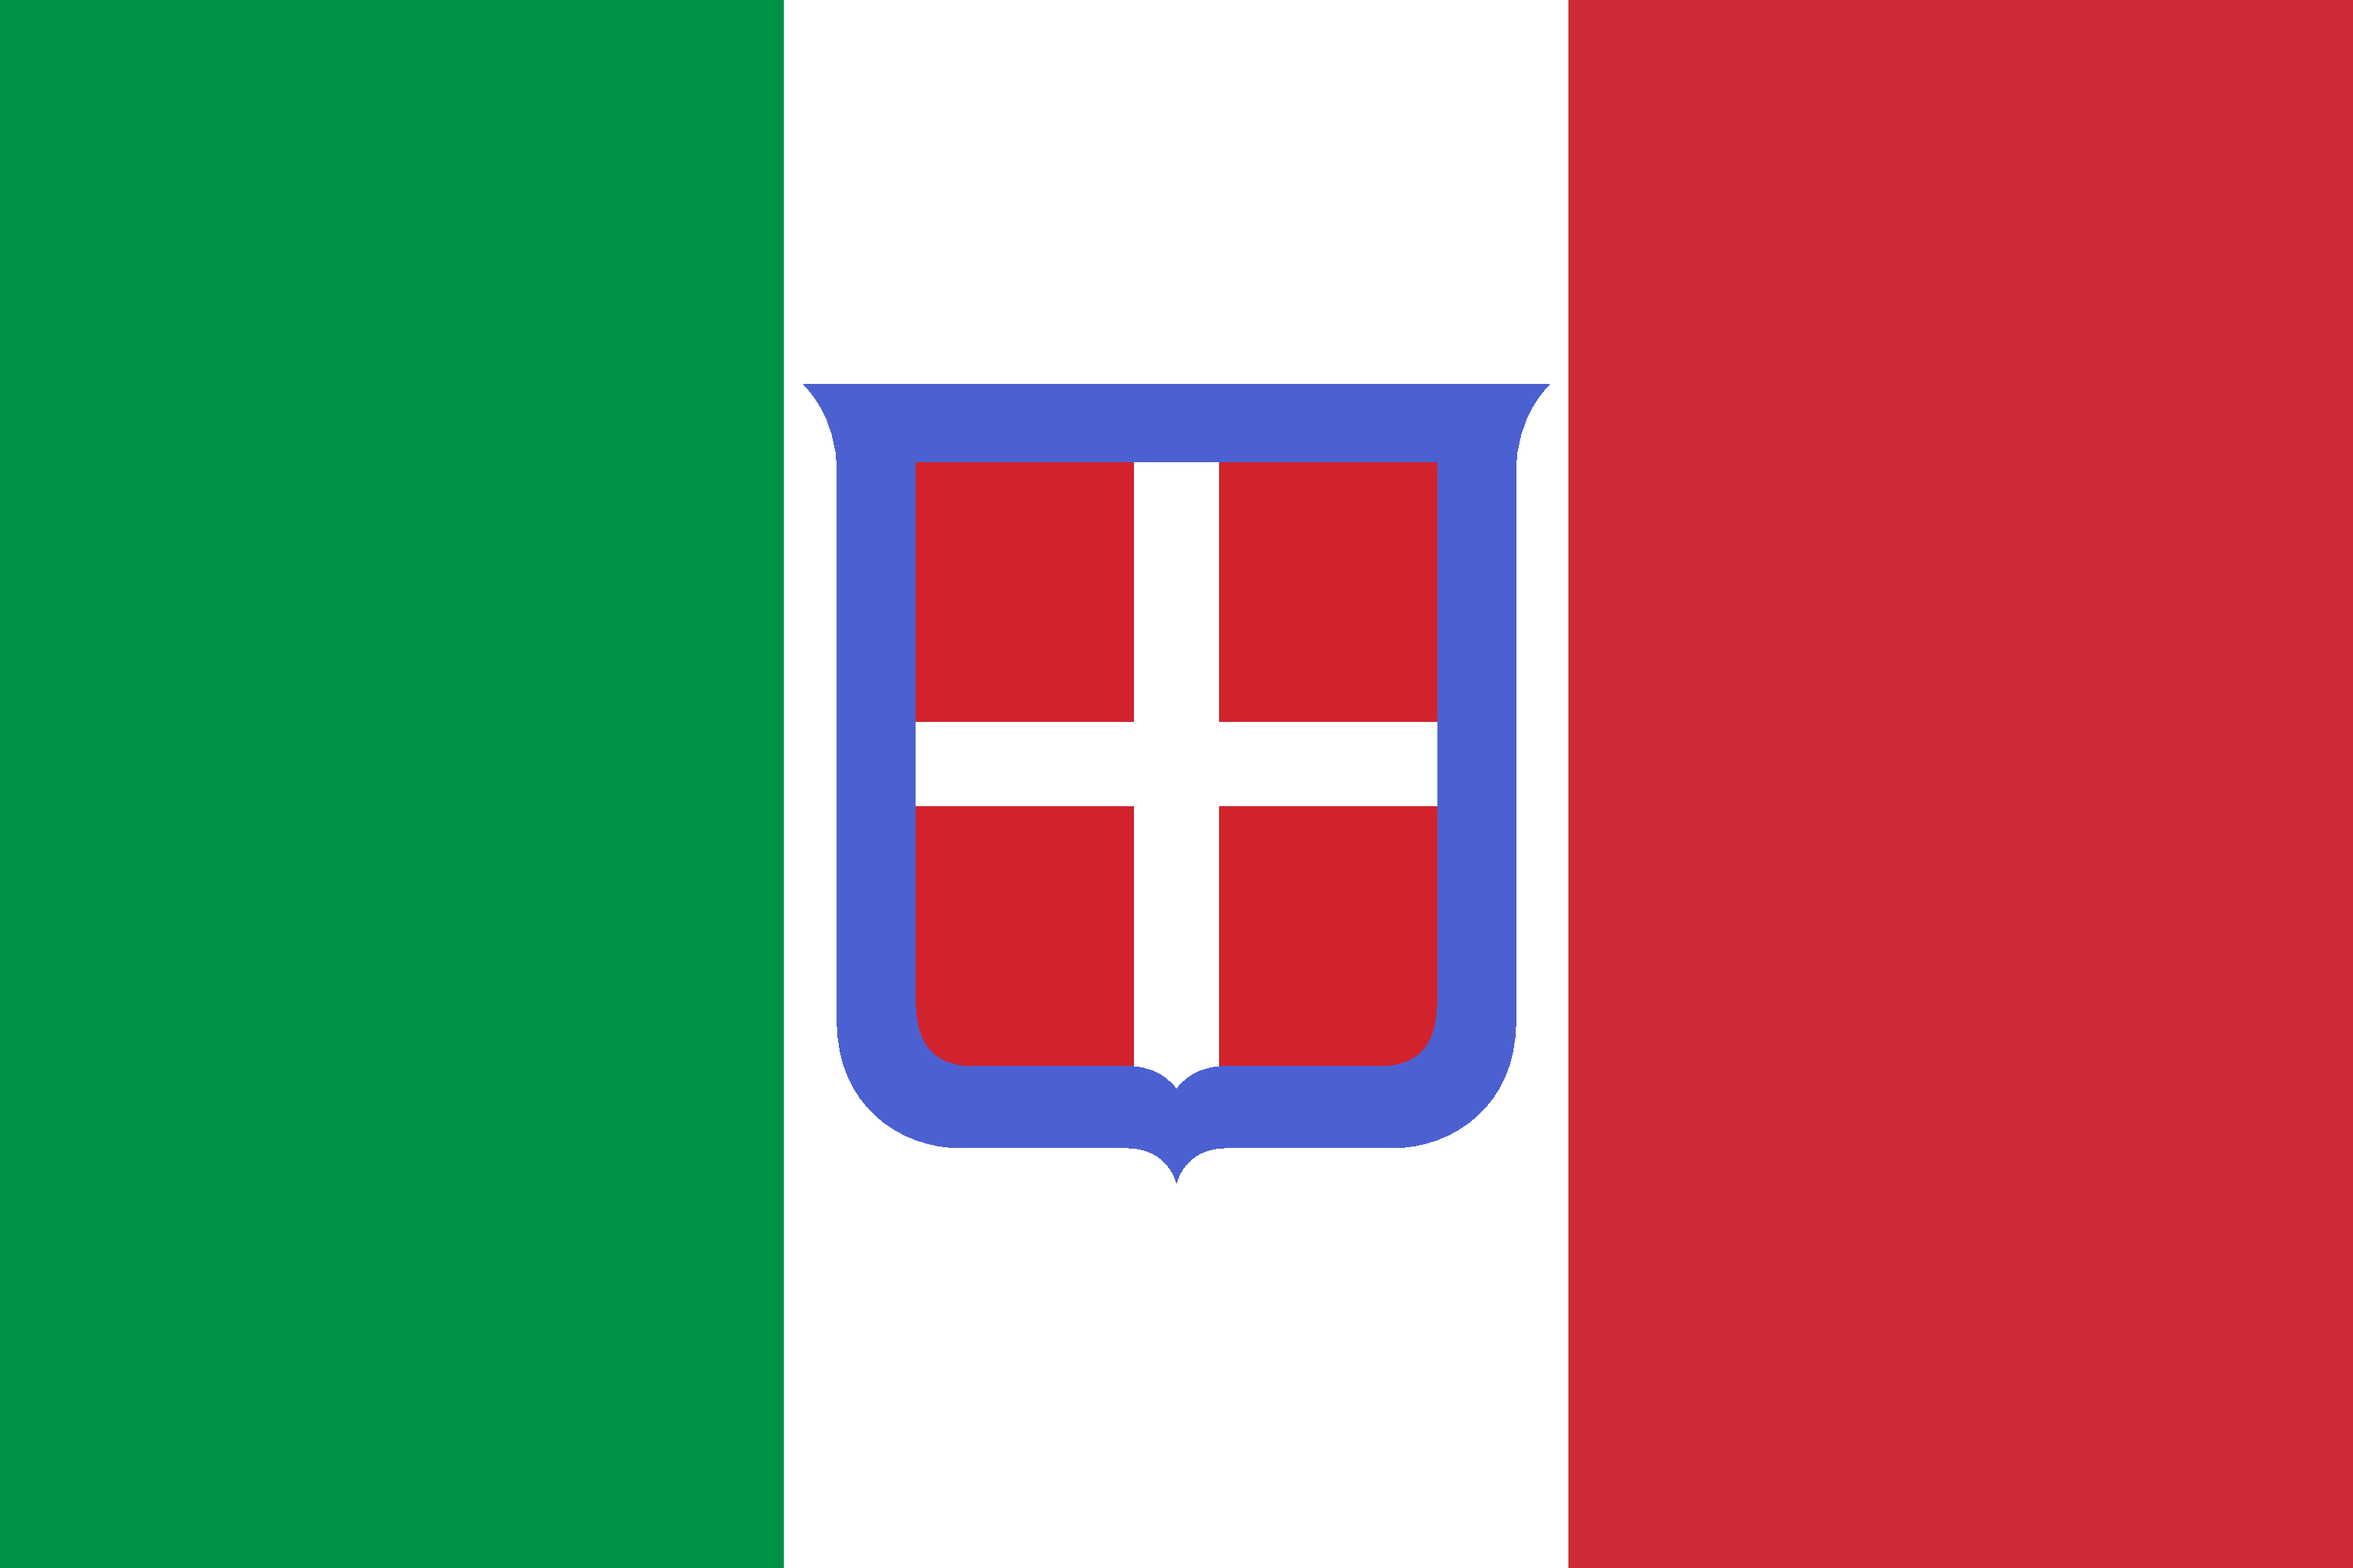
\includegraphics[width=1.0\linewidth]{Annexes/friseChronologique/img/Flag_of_Italy_281861E28093194629.pdf}
                \captionsetup{labelformat=empty}\refDrapeau{Drapeau Italy 281861E28093194629}{frise:Flag_of_Italy_281861E28093194629.pdf}
            \end{figure}
            
            \centering\mdiMilitaire
        \end{minipage}
    &
        \begin{minipage}{.65\textwidth}
            \textbf{23 novembre 1911} - \textbf{Premier usage d'avions au combat}
            
            Les Italiens sont les premiers à utiliser des avions au combat à l'occasion de la guerre de Libye.

Les Italiens utilisent des avions Blériot XI, Nieuport, Farman et Etrich Taube
            \begin{figure}[H]
                \legende{Avion italien lors d'un attaque en Libye}{frise:Italian_Nieuport_IV_attacking_Ottoman_forces_in_Libya_1911_or_1912.jpg}
            \end{figure}
        \end{minipage}
    &
        \begin{minipage}{.275\textwidth}
            \begin{figure}[H]
                \centering
                \includegraphics[width=1.0\linewidth]{Annexes/friseChronologique/img/Italian_Nieuport_IV_attacking_Ottoman_forces_in_Libya_1911_or_1912.jpg}
            \end{figure}
        \end{minipage}
    \end{tabular}
\end{table}
\begin{table}[H]
    \centering
    \begin{tabular}{c l c}
        \begin{minipage}{.075\textwidth}
            \begin{figure}[H]
                \centering
                
\includegraphics[width=1.0\linewidth]{Annexes/friseChronologique/img/Flag_of_France.pdf}
                \captionsetup{labelformat=empty}\refDrapeau{Drapeau France}{frise:Flag_of_France.pdf}
            \end{figure}
        \end{minipage}
    &
        \begin{minipage}{.65\textwidth}
            \textbf{21 septembre 1913} - \textbf{Adolphe Pégoud : premier looping}
            
            Le 19 août 1913, Adolphe Pegoud est le premier pilote de l'histoire à utiliser un parachute pour abandonner un avion en perdition.

L'histoire raconte que l'avion qu'il venait de quitter aurait alors effecuté un looping. C'est de cet événément qu'Adolphe Pegoud aurait tiré l'idée de réaliser un looping à bord de son avion, chose qu'il réalise le 21 septembre.
            \begin{figure}[H]
                \legende{Carte postale allemande illustrant le looping d'Adolphe Pegoud.}{frise:Adolphe_PC3A9goud_Looping.jpg}
            \end{figure}
        \end{minipage}
    &
        \begin{minipage}{.275\textwidth}
            \begin{figure}[H]
                \centering
                \includegraphics[width=1.0\linewidth]{Annexes/friseChronologique/img/Adolphe_PC3A9goud_Looping.jpg}
            \end{figure}
        \end{minipage}
    \end{tabular}
\end{table}
\section{La première guerre mondiale}

\begin{table}[H]
    \centering
    \begin{tabular}{c l c}
        \begin{minipage}{.075\textwidth}
            \begin{figure}[H]
                \centering
                
\includegraphics[width=1.0\linewidth]{Annexes/friseChronologique/img/Flag_of_France.pdf}
                \captionsetup{labelformat=empty}\refDrapeau{Drapeau France}{frise:Flag_of_France.pdf}
            \end{figure}
        \end{minipage}
    &
        \begin{minipage}{.65\textwidth}
            \textbf{1914} - \textbf{René Fonck, as des as}
            
            René Fonck est le pilote français ayant le plus grand nombre de victoires aériennes (75). Il est surnomé "l'as des as"
            \begin{figure}[H]
                \legende{Portrait de René Fonck}{frise:RenC3A9_Fonck_02.jpg}
            \end{figure}
        \end{minipage}
    &
        \begin{minipage}{.275\textwidth}
            \begin{figure}[H]
                \centering
                \includegraphics[width=1.0\linewidth]{Annexes/friseChronologique/img/RenC3A9_Fonck_02.jpg}
            \end{figure}
        \end{minipage}
    \end{tabular}
\end{table}
\begin{table}[H]
    \centering
    \begin{tabular}{c l c}
        \begin{minipage}{.075\textwidth}
            \begin{figure}[H]
                \centering
                
\includegraphics[width=1.0\linewidth]{Annexes/friseChronologique/img/Flag_of_Germany_281867E28093191829.pdf}
                \captionsetup{labelformat=empty}\refDrapeau{Drapeau Germany 281867E28093191829}{frise:Flag_of_Germany_281867E28093191829.pdf}
            \end{figure}
        \end{minipage}
    &
        \begin{minipage}{.65\textwidth}
            \textbf{1914} - \textbf{Manfred von Richtoffen, as de la première guerre mondiale}
            
            Manfred von Richtoffen, pilote allemand, dispose du plus grand nombre de victoires confirmées (80) lors du premier conflit mondial.

Il est connu sous le nom du Baron rouge
            \begin{figure}[H]
                \legende{Le Baron Rouge, Manfred von Richtoffen}{frise:Manfred_von_Richthofen.jpg}
            \end{figure}
        \end{minipage}
    &
        \begin{minipage}{.275\textwidth}
            \begin{figure}[H]
                \centering
                \includegraphics[width=1.0\linewidth]{Annexes/friseChronologique/img/Manfred_von_Richthofen.jpg}
            \end{figure}
        \end{minipage}
    \end{tabular}
\end{table}
\begin{table}[H]
    \centering
    \begin{tabular}{c l c}
        \begin{minipage}{.075\textwidth}
            \begin{figure}[H]
                \centering
                \includegraphics[width=1.0\linewidth]{Annexes/friseChronologique/img/Flag_of_Germany_281867E28093191829.pdf}
                \captionsetup{labelformat=empty}\refDrapeau{Drapeau Germany 281867E28093191829}{frise:Flag_of_Germany_281867E28093191829.pdf}
            \end{figure}
        \end{minipage}
    &
        \begin{minipage}{.65\textwidth}
            \textbf{12 décembre 1915} - \textbf{Premier vol du Junker J1, premier avion entièrement métallique}
            
            
            \begin{figure}[H]
                \legende{Junker J1}{frise:Junkers_J_1_at_DC3B6beritz_1915.jpg}
            \end{figure}
        \end{minipage}
    &
        \begin{minipage}{.275\textwidth}
            \begin{figure}[H]
                \centering
                \includegraphics[width=1.0\linewidth]{Annexes/friseChronologique/img/Junkers_J_1_at_DC3B6beritz_1915.jpg}
            \end{figure}
        \end{minipage}
    \end{tabular}
\end{table}
\begin{table}[H]
    \centering
    \begin{tabular}{c l c}
        \begin{minipage}{.075\textwidth}
            \begin{figure}[H]
                \centering
                \includegraphics[width=1.0\linewidth]{Annexes/friseChronologique/img/Flag_of_France.pdf}
                \captionsetup{labelformat=empty}\refDrapeau{Drapeau France}{frise:Flag_of_France.pdf}
            \end{figure}
        \end{minipage}
    &
        \begin{minipage}{.65\textwidth}
            \textbf{01 février 1916} - \textbf{Marcel Bloch concoit l'hélice Éclair}
            
            Marcel Dassault (qui s'appelait alors Marcel Bloch) dessine l'hélice Éclair. Cette hélice à marqué l'histoire car elle est très performante. Elle sera produite à plus de 4000 exemplaire et montée sur 10 des 20 avions les plus perfomants de l'armée française de cette époque.
            \begin{figure}[H]
                \legende{Le SPAD VII de Georges Guynemer, équipé de l'hélice Eclair}{frise:Georges_Guynemer27s_SPAD_VII2C_Musee_de_l27Air_et_de_l27Espace2C_Le_Bourget2C_Paris._28812284872329.jpg}
            \end{figure}
        \end{minipage}
    &
        \begin{minipage}{.275\textwidth}
            \begin{figure}[H]
                \centering
                \includegraphics[width=1.0\linewidth]{Annexes/friseChronologique/img/Georges_Guynemer27s_SPAD_VII2C_Musee_de_l27Air_et_de_l27Espace2C_Le_Bourget2C_Paris._28812284872329.jpg}
            \end{figure}
        \end{minipage}
    \end{tabular}
\end{table}
\section{L'entre 2 guerres}

\begin{table}[H]
    \centering
    \begin{tabular}{c l c}
        \begin{minipage}{.075\textwidth}
            \begin{figure}[H]
                \centering
                \includegraphics[width=1.0\linewidth]{Annexes/friseChronologique/img/Flag_of_France.pdf}
                \captionsetup{labelformat=empty}\refDrapeau{Drapeau France}{frise:Flag_of_France.pdf}
            \end{figure}
        \end{minipage}
    &
        \begin{minipage}{.65\textwidth}
            \textbf{25 décembre 1918} - \textbf{Georges Latécoère lance l'Aéropostale}
            
            L'Aéropostale est le transport de courrier et frets (colis) par voie aérienne.

Le 25 décembre 1918, il ouvre la ligne entre Toulouse et Barcelone.

Dès 1919, la ligne est étendue jusqu'à Casablanca. Elle sera par la suite prolongée jusqu'à Dakar puis l'Amérique du Sud via Rio au Brésil, puis jusqu'à Buenos-Aires et Santiago du Chili
            \begin{figure}[H]
                \legende{Carte illustrant les lignes de l'aéropostale entre la France et l'Amérique du Sud, en 1930.}{frise:AC3A9ropostale._AmC3A9rique_du_Sud._Maroc_-_AlgC3A9rie_-_Afrique_Occidentale_FranC3A7aise_-_affiche_-_btv1b10104627j.jpg}
            \end{figure}
        \end{minipage}
    &
        \begin{minipage}{.275\textwidth}
            \begin{figure}[H]
                \centering
                \includegraphics[width=1.0\linewidth]{Annexes/friseChronologique/img/AC3A9ropostale._AmC3A9rique_du_Sud._Maroc_-_AlgC3A9rie_-_Afrique_Occidentale_FranC3A7aise_-_affiche_-_btv1b10104627j.jpg}
            \end{figure}
        \end{minipage}
    \end{tabular}
\end{table}
\begin{table}[H]
    \centering
    \begin{tabular}{c l c}
        \begin{minipage}{.075\textwidth}
            \begin{figure}[H]
                \centering
                \includegraphics[width=1.0\linewidth]{Annexes/friseChronologique/img/Flag_of_France.pdf}
                \captionsetup{labelformat=empty}\refDrapeau{Drapeau France}{frise:Flag_of_France.pdf}
            \end{figure}
            
            \centering\mdiFemale
        \end{minipage}
    &
        \begin{minipage}{.65\textwidth}
            \textbf{01 avril 1921} - \textbf{Adrienne Bolland, première femme à traverser la Cordillière des Andes}
            
            Adrienne Bolland traverse la Cordillière en Caudron G3 en 4h15
            \begin{figure}[H]
                \legende{Adrienne Bolland faisant la couverture du magazine argentin El Gráfico le 19 mars 1921}{frise:Adrienne_Bolland_-_El_GrC3A1fico_91.jpg}
            \end{figure}
        \end{minipage}
    &
        \begin{minipage}{.275\textwidth}
            \begin{figure}[H]
                \centering
                \includegraphics[width=1.0\linewidth]{Annexes/friseChronologique/img/Adrienne_Bolland_-_El_GrC3A1fico_91.jpg}
            \end{figure}
        \end{minipage}
    \end{tabular}
\end{table}
\begin{table}[H]
    \centering
    \begin{tabular}{c l c}
        \begin{minipage}{.075\textwidth}
            \begin{figure}[H]
                \centering
                \includegraphics[width=1.0\linewidth]{Annexes/friseChronologique/img/Flag_of_Spain.pdf}
                \captionsetup{labelformat=empty}\refDrapeau{Drapeau Spain}{frise:Flag_of_Spain.pdf}
            \end{figure}
        \end{minipage}
    &
        \begin{minipage}{.65\textwidth}
            \textbf{1923} - \textbf{Premier vol d'un autogire}
            
            Juan de la Cierva effectue le premier vol d'un autogire
            \begin{figure}[H]
                \legende{L'autogire C-6 de Juan de la Cierva (1925)}{frise:Autogyro_at_Farnborough2C_1925_28Our_Generation2C_193829.jpg}
            \end{figure}
        \end{minipage}
    &
        \begin{minipage}{.275\textwidth}
            \begin{figure}[H]
                \centering
                \includegraphics[width=1.0\linewidth]{Annexes/friseChronologique/img/Autogyro_at_Farnborough2C_1925_28Our_Generation2C_193829.jpg}
            \end{figure}
        \end{minipage}
    \end{tabular}
\end{table}
\begin{table}[H]
    \centering
    \begin{tabular}{c l c}
        \begin{minipage}{.075\textwidth}
            \begin{figure}[H]
                \centering
                \includegraphics[width=1.0\linewidth]{Annexes/friseChronologique/img/Flag_of_the_United_States_28DDD-F-416E_specifications29.pdf}
                \captionsetup{labelformat=empty}\refDrapeau{Drapeau the United States 28DDD-F-416E specifications29}{frise:Flag_of_the_United_States_28DDD-F-416E_specifications29.pdf}
            \end{figure}
        \end{minipage}
    &
        \begin{minipage}{.65\textwidth}
            \textbf{20 mai 1927} - \textbf{Charles Lindbergh réalise le premier vol transaltantique }
            
            Charles Lindbergh réalise le premier vol transaltantique entre New-York et Paris, à bord de son avion,  le Spirit of Saint-Louis
            \begin{figure}[H]
                \legende{}{frise:Col_Charles_Lindbergh2C_original2C_hec.21329.jpg}
            \end{figure}
        \end{minipage}
    &
        \begin{minipage}{.275\textwidth}
            \begin{figure}[H]
                \centering
                \includegraphics[width=1.0\linewidth]{Annexes/friseChronologique/img/Col_Charles_Lindbergh2C_original2C_hec.21329.jpg}
            \end{figure}
        \end{minipage}
    \end{tabular}
\end{table}
\begin{table}[H]
    \centering
    \begin{tabular}{c l c}
        \begin{minipage}{.075\textwidth}
            \begin{figure}[H]
                \centering
                \includegraphics[width=1.0\linewidth]{Annexes/friseChronologique/img/Flag_of_France.pdf}
                \captionsetup{labelformat=empty}\refDrapeau{Drapeau France}{frise:Flag_of_France.pdf}
            \end{figure}
            
            \centering\mdiFemale
            
            \centering\faTrophy
        \end{minipage}
    &
        \begin{minipage}{.65\textwidth}
            \textbf{13 juillet 1928} - \textbf{Maryse Bastié, première recordwomen de distance}
            
            
            \begin{figure}[H]
                \legende{L'aviatrice française Maryse Bastié à ses débuts.}{frise:Maryse_bastie.jpg}
            \end{figure}
        \end{minipage}
    &
        \begin{minipage}{.275\textwidth}
            \begin{figure}[H]
                \centering
                \includegraphics[width=1.0\linewidth]{Annexes/friseChronologique/img/Maryse_bastie.jpg}
            \end{figure}
        \end{minipage}
    \end{tabular}
\end{table}
\begin{table}[H]
    \centering
    \begin{tabular}{c l c}
        \begin{minipage}{.075\textwidth}
            \begin{figure}[H]
                \centering
                \includegraphics[width=1.0\linewidth]{Annexes/friseChronologique/img/Flag_of_the_United_States_28DDD-F-416E_specifications29.pdf}
                \captionsetup{labelformat=empty}\refDrapeau{Drapeau the United States 28DDD-F-416E specifications29}{frise:Flag_of_the_United_States_28DDD-F-416E_specifications29.pdf}
            \end{figure}
            
            \centering\mdiFemale
        \end{minipage}
    &
        \begin{minipage}{.65\textwidth}
            \textbf{20 mai 1932} - \textbf{Amelia Earhart traverse l'Atlantique en solitaire}
            
            En 1928, Amelia Earhart traverse l'Atlantique avec Wilmer Stultz et Louis Gordon. Elle devient ainsi la première femme à effectuer une transatlantique en avion.

Le 20 mai 1932, elle réitère la traversée, mais cette fois ci, seule. Elle effectue en une quinzaine d'heures sur son Lockheed Vega la traversée entre entre le Canada et l'Irlande du Nord.
            \begin{figure}[H]
                \legende{Amelia Earhart en 1935}{frise:Amelia_Earhart_1935.jpg}
            \end{figure}
        \end{minipage}
    &
        \begin{minipage}{.275\textwidth}
            \begin{figure}[H]
                \centering
                \includegraphics[width=1.0\linewidth]{Annexes/friseChronologique/img/Amelia_Earhart_1935.jpg}
            \end{figure}
        \end{minipage}
    \end{tabular}
\end{table}
\begin{table}[H]
    \centering
    \begin{tabular}{c l c}
        \begin{minipage}{.075\textwidth}
            \begin{figure}[H]
                \centering
                \includegraphics[width=1.0\linewidth]{Annexes/friseChronologique/img/Flag_of_France.pdf}
                \captionsetup{labelformat=empty}\refDrapeau{Drapeau France}{frise:Flag_of_France.pdf}
            \end{figure}
        \end{minipage}
    &
        \begin{minipage}{.65\textwidth}
            \textbf{1933} - \textbf{Création de la compagnie Air France}
            
            
            \begin{figure}[H]
                \legende{Un Lockheed Super Constellation d'Air France à Heathrow en 1955}{frise:Lockheed_L1049_F-BGNG_Air_France_LAP_08.04.55_edited-2.jpg}
            \end{figure}
        \end{minipage}
    &
        \begin{minipage}{.275\textwidth}
            \begin{figure}[H]
                \centering
                \includegraphics[width=1.0\linewidth]{Annexes/friseChronologique/img/Lockheed_L1049_F-BGNG_Air_France_LAP_08.04.55_edited-2.jpg}
            \end{figure}
        \end{minipage}
    \end{tabular}
\end{table}
\begin{table}[H]
    \centering
    \begin{tabular}{c l c}
        \begin{minipage}{.075\textwidth}
            \begin{figure}[H]
                \centering
                \includegraphics[width=1.0\linewidth]{Annexes/friseChronologique/img/Flag_of_the_United_Kingdom_283-529.pdf}
                \captionsetup{labelformat=empty}\refDrapeau{Drapeau the United Kingdom 283-529}{frise:Flag_of_the_United_Kingdom_283-529.pdf}
            \end{figure}
            
            \centering\mdiBrevet
        \end{minipage}
    &
        \begin{minipage}{.65\textwidth}
            \textbf{1935} - \textbf{Robert Watson-Watt invente le radar}
            
            Le britannique Robert Watson-Watt dépose un brevet pour le radar, qui permet de détecter à distance des objets, et notamment des avions. Durant la seconde guerre mondiale, cett invention donnera un avantage décisif aux britanniques durant la bataille d'Angleterre (1940)
            \begin{figure}[H]
                \legende{Composant d'un radar conçu par Robet Watson-Watt}{frise:Watson_Radar.jpg}
            \end{figure}
        \end{minipage}
    &
        \begin{minipage}{.275\textwidth}
            \begin{figure}[H]
                \centering
                \includegraphics[width=1.0\linewidth]{Annexes/friseChronologique/img/Watson_Radar.jpg}
            \end{figure}
        \end{minipage}
    \end{tabular}
\end{table}
\begin{table}[H]
    \centering
    \begin{tabular}{c l c}
        \begin{minipage}{.075\textwidth}
            \begin{figure}[H]
                \centering
                \includegraphics[width=1.0\linewidth]{Annexes/friseChronologique/img/Flag_of_Germany.pdf}
                \captionsetup{labelformat=empty}\refDrapeau{Drapeau Germany}{frise:Flag_of_Germany.pdf}
            \end{figure}
        \end{minipage}
    &
        \begin{minipage}{.65\textwidth}
            \textbf{1936} - \textbf{Premier vol d'un hélicoptère}
            
            Le Focke-Wulf Fw 61 est le premier hélicoptère ayant effecuté un vol totalement contrôlé
            \begin{figure}[H]
                \legende{Le Focke-Wulf Fw 61 en vol}{frise:Fw_61_V.JPG}
            \end{figure}
        \end{minipage}
    &
        \begin{minipage}{.275\textwidth}
            \begin{figure}[H]
                \centering
                \includegraphics[width=1.0\linewidth]{Annexes/friseChronologique/img/Fw_61_V.JPG}
            \end{figure}
        \end{minipage}
    \end{tabular}
\end{table}
\begin{table}[H]
    \centering
    \begin{tabular}{c l c}
        \begin{minipage}{.075\textwidth}
            \begin{figure}[H]
                \centering
                \includegraphics[width=1.0\linewidth]{Annexes/friseChronologique/img/Flag_of_the_United_Kingdom_283-529.pdf}
                \captionsetup{labelformat=empty}\refDrapeau{Drapeau the United Kingdom 283-529}{frise:Flag_of_the_United_Kingdom_283-529.pdf}
            \end{figure}
        \end{minipage}
    &
        \begin{minipage}{.65\textwidth}
            \textbf{05 mars 1936} - \textbf{Premier vol du Spitfire}
            
            Le Supermarine Spitfire est un chasseur à hélice. Il sera considéré comme le meilleur avion de la seconde guerre mondiale.
            \begin{figure}[H]
                \legende{Un Spitfire}{frise:Ray_Flying_Legends_2005-1.jpg}
            \end{figure}
        \end{minipage}
    &
        \begin{minipage}{.275\textwidth}
            \begin{figure}[H]
                \centering
                \includegraphics[width=1.0\linewidth]{Annexes/friseChronologique/img/Ray_Flying_Legends_2005-1.jpg}
            \end{figure}
        \end{minipage}
    \end{tabular}
\end{table}
\section{La seconde guerre mondiale}

\begin{table}[H]
    \centering
    \begin{tabular}{c l c}
        \begin{minipage}{.075\textwidth}
            \begin{figure}[H]
                \centering
                \includegraphics[width=1.0\linewidth]{Annexes/friseChronologique/img/Flag_of_Germany_281935E28093194529.pdf}
                \captionsetup{labelformat=empty}\refDrapeau{Drapeau Germany 281935E28093194529}{frise:Flag_of_Germany_281935E28093194529.pdf}
            \end{figure}
            
            \centering\mdiMilitaire
        \end{minipage}
    &
        \begin{minipage}{.65\textwidth}
            \textbf{18 juillet 1942} - \textbf{Le Messerschmitt Me 262, premier chasseur à réaction}
            
            Premier chasseur à réaction de l'Histoire, sa mise au point fut cependant longue et son entrée en service dans la Luftwaffe (armée de l'air allemande) en avril 1944 (donc à la fin de la guerre) impliquera que cet avion aura un rôle mineur dans le second conflit mondial.
            \begin{figure}[H]
                \legende{Un Messerschmitt Me 262}{frise:Messerschmitt_Me_262A_at_the_National_Museum_of_the_USAF.jpg}
            \end{figure}
        \end{minipage}
    &
        \begin{minipage}{.275\textwidth}
            \begin{figure}[H]
                \centering
                \includegraphics[width=1.0\linewidth]{Annexes/friseChronologique/img/Messerschmitt_Me_262A_at_the_National_Museum_of_the_USAF.jpg}
            \end{figure}
        \end{minipage}
    \end{tabular}
\end{table}
\begin{table}[H]
    \centering
    \begin{tabular}{c l c}
        \begin{minipage}{.075\textwidth}
            \begin{figure}[H]
                \centering
                \includegraphics[width=1.0\linewidth]{Annexes/friseChronologique/img/Flag_of_Germany_281935E28093194529.pdf}
                \captionsetup{labelformat=empty}\refDrapeau{Drapeau Germany 281935E28093194529}{frise:Flag_of_Germany_281935E28093194529.pdf}
            \end{figure}
            
            \centering\mdiRocket
            
            \centering\mdiMilitaire
        \end{minipage}
    &
        \begin{minipage}{.65\textwidth}
            \textbf{03 octobre 1942} - \textbf{Premier vol d'un missile balistique V2}
            
            L'Allemagne nazie réalise le premier lancement réussi d'un missile V2. Ce type de missile, mis au point sous l'égide de Wener Von Braun, sont des fusées utilisées pour bombarder principalement le Royaume-Unis et la Belgique.
            \begin{figure}[H]
                \legende{Réplique de missile V2, Usedom, Allemagne}{frise:La2-v2.jpg}
            \end{figure}
        \end{minipage}
    &
        \begin{minipage}{.275\textwidth}
            \begin{figure}[H]
                \centering
                \includegraphics[width=1.0\linewidth]{Annexes/friseChronologique/img/La2-v2.jpg}
            \end{figure}
        \end{minipage}
    \end{tabular}
\end{table}
\begin{table}[H]
    \centering
    \begin{tabular}{c l c}
        \begin{minipage}{.075\textwidth}
            \begin{figure}[H]
                \centering
                \includegraphics[width=1.0\linewidth]{Annexes/friseChronologique/img/Flag_of_the_United_States_28DDD-F-416E_specifications29.pdf}
                \captionsetup{labelformat=empty}\refDrapeau{Drapeau the United States 28DDD-F-416E specifications29}{frise:Flag_of_the_United_States_28DDD-F-416E_specifications29.pdf}
            \end{figure}
            
            \centering\mdiFemale
        \end{minipage}
    &
        \begin{minipage}{.65\textwidth}
            \textbf{05 août 1943} - \textbf{Jacqueline Cochran crée le Women Airforce Service Pilots}
            
            
        \end{minipage}
    &
        \begin{minipage}{.275\textwidth}
            \begin{figure}[H]
                \centering
                \includegraphics[width=1.0\linewidth]{Annexes/friseChronologique/vide.pdf}
            \end{figure}
        \end{minipage}
    \end{tabular}
\end{table}
\begin{table}[H]
    \centering
    \begin{tabular}{c l c}
        \begin{minipage}{.075\textwidth}
            \begin{figure}[H]
                \centering
                \includegraphics[width=1.0\linewidth]{Annexes/friseChronologique/img/Flag_of_ICAO.pdf}
                \captionsetup{labelformat=empty}\refDrapeau{Drapeau ICAO}{frise:Flag_of_ICAO.pdf}
            \end{figure}
        \end{minipage}
    &
        \begin{minipage}{.65\textwidth}
            \textbf{07 décembre 1944} - \textbf{Création de l'OACI}
            
            L'Organisation de l'Aviation Civile Internationale est créée en 1944 par la convention de Chicago.

 Son rôle est de participer à l’élaboration des politiques et des normes qui permettent la standardisation du transport aéronautique international.

Le conseil de l’OACI adopte les normes et recommandations règlementant la navigation, le partage des fréquences radio, les brevets du personnel d'aviation, la circulation aérienne, etc. Il définit aussi les protocoles à suivre lors des enquêtes sur les accidents aériens, protocoles qui sont respectés par les pays signataires de la Convention de Chicago.

Cette réglementation produite par l'OACI a permis depuis la fin de la Seconde Guerre mondiale la mise en œuvre du transport aérien, tant des personnes que des biens, au niveau mondial, grâce à des recommandations suivies par l'ensemble des États membres, des équipementiers de l'aéronautique et fabricants d'avions, des établissements responsables d’aéroports...
            \begin{figure}[H]
                \legende{Siège de l'OACI à Montréal}{frise:La_Maison_de_l-OACI_-_11a.jpg}
            \end{figure}
        \end{minipage}
    &
        \begin{minipage}{.275\textwidth}
            \begin{figure}[H]
                \centering
                \includegraphics[width=1.0\linewidth]{Annexes/friseChronologique/img/La_Maison_de_l-OACI_-_11a.jpg}
            \end{figure}
        \end{minipage}
    \end{tabular}
\end{table}
\section{L'age d'or de la réaction et la guerre froide}

\begin{table}[H]
    \centering
    \begin{tabular}{c l c}
        \begin{minipage}{.075\textwidth}
            \begin{figure}[H]
                \centering
                \includegraphics[width=1.0\linewidth]{Annexes/friseChronologique/img/Flag_of_the_United_States_28DDD-F-416E_specifications29.pdf}
                \captionsetup{labelformat=empty}\refDrapeau{Drapeau the United States 28DDD-F-416E specifications29}{frise:Flag_of_the_United_States_28DDD-F-416E_specifications29.pdf}
            \end{figure}
        \end{minipage}
    &
        \begin{minipage}{.65\textwidth}
            \textbf{14 octobre 1947} - \textbf{Chuck Yeager franchit le mur du son}
            
            Chuck Yeager devient le premier humain à franchir le mur du son, à bord du Bell X1.
            \begin{figure}[H]
                \legende{L'avion fusée Bell X1}{frise:Bell_X-1_46-062_28in_flight29.jpg}
            \end{figure}
        \end{minipage}
    &
        \begin{minipage}{.275\textwidth}
            \begin{figure}[H]
                \centering
                \includegraphics[width=1.0\linewidth]{Annexes/friseChronologique/img/Bell_X-1_46-062_28in_flight29.jpg}
            \end{figure}
        \end{minipage}
    \end{tabular}
\end{table}
\begin{table}[H]
    \centering
    \begin{tabular}{c l c}
        \begin{minipage}{.075\textwidth}
            \begin{figure}[H]
                \centering
                \includegraphics[width=1.0\linewidth]{Annexes/friseChronologique/img/Flag_of_France.pdf}
                \captionsetup{labelformat=empty}\refDrapeau{Drapeau France}{frise:Flag_of_France.pdf}
            \end{figure}
        \end{minipage}
    &
        \begin{minipage}{.65\textwidth}
            \textbf{1953} - \textbf{Création de la patrouille de France}
            
            
            \begin{figure}[H]
                \legende{Photo récente de la Patrouille de France, sur AlphaJet}{frise:Alphajet_5_en_passage_au_meeting_d27Orange_2019.jpg}
            \end{figure}
        \end{minipage}
    &
        \begin{minipage}{.275\textwidth}
            \begin{figure}[H]
                \centering
                \includegraphics[width=1.0\linewidth]{Annexes/friseChronologique/img/Alphajet_5_en_passage_au_meeting_d27Orange_2019.jpg}
            \end{figure}
        \end{minipage}
    \end{tabular}
\end{table}
\begin{table}[H]
    \centering
    \begin{tabular}{c l c}
        \begin{minipage}{.075\textwidth}
            \begin{figure}[H]
                \centering
                \includegraphics[width=1.0\linewidth]{Annexes/friseChronologique/img/Flag_of_the_United_States_28DDD-F-416E_specifications29.pdf}
                \captionsetup{labelformat=empty}\refDrapeau{Drapeau the United States 28DDD-F-416E specifications29}{frise:Flag_of_the_United_States_28DDD-F-416E_specifications29.pdf}
            \end{figure}
            
            \centering\mdiFemale
        \end{minipage}
    &
        \begin{minipage}{.65\textwidth}
            \textbf{18 mai 1953} - \textbf{Jacqueline Cochran, première femme à passer le mur du son}
            
            
            \begin{figure}[H]
                \legende{Jacqueline Cochran à bord de son Canadair Sabre 3, avion dans lequel elle franchira le mur du son. Sur cette photo, elle parle avec Chuck Yeager}{frise:Cochrane_with_Yeager.jpg}
            \end{figure}
        \end{minipage}
    &
        \begin{minipage}{.275\textwidth}
            \begin{figure}[H]
                \centering
                \includegraphics[width=1.0\linewidth]{Annexes/friseChronologique/img/Cochrane_with_Yeager.jpg}
            \end{figure}
        \end{minipage}
    \end{tabular}
\end{table}
\begin{table}[H]
    \centering
    \begin{tabular}{c l c}
        \begin{minipage}{.075\textwidth}
            \begin{figure}[H]
                \centering
                \includegraphics[width=1.0\linewidth]{Annexes/friseChronologique/img/Flag_of_France.pdf}
                \captionsetup{labelformat=empty}\refDrapeau{Drapeau France}{frise:Flag_of_France.pdf}
            \end{figure}
            
            \centering\mdiFemale
        \end{minipage}
    &
        \begin{minipage}{.65\textwidth}
            \textbf{15 août 1953} - \textbf{Jacqueline Auriol, première femme européenne à franchir le mur du son}
            
            Durant toute sa vie, Jacqueline Auriol sera en concurrence serrée avec l'aviatrice Jacqueline Cochran. Ces 2 femmes sont souvent désignées comme "les Jacquelines".
            \begin{figure}[H]
                \legende{Jacqueline Auriol en 1947}{frise:Auriol_Harcourt_1947_2.jpg}
            \end{figure}
        \end{minipage}
    &
        \begin{minipage}{.275\textwidth}
            \begin{figure}[H]
                \centering
                \includegraphics[width=1.0\linewidth]{Annexes/friseChronologique/img/Auriol_Harcourt_1947_2.jpg}
            \end{figure}
        \end{minipage}
    \end{tabular}
\end{table}
\begin{table}[H]
    \centering
    \begin{tabular}{c l c}
        \begin{minipage}{.075\textwidth}
            \begin{figure}[H]
                \centering
                \includegraphics[width=1.0\linewidth]{Annexes/friseChronologique/img/Flag_of_the_Soviet_Union.pdf}
                \captionsetup{labelformat=empty}\refDrapeau{Drapeau the Soviet Union}{frise:Flag_of_the_Soviet_Union.pdf}
            \end{figure}
        \end{minipage}
    &
        \begin{minipage}{.65\textwidth}
            \textbf{1957} - \textbf{Spoutnik 1, premier satellite artificiel}
            
            Lancé par l'URSS
            \begin{figure}[H]
                \legende{Une réplique de Spoutnik 1}{frise:Sputnik_asm.jpg}
            \end{figure}
        \end{minipage}
    &
        \begin{minipage}{.275\textwidth}
            \begin{figure}[H]
                \centering
                \includegraphics[width=1.0\linewidth]{Annexes/friseChronologique/img/Sputnik_asm.jpg}
            \end{figure}
        \end{minipage}
    \end{tabular}
\end{table}
\begin{table}[H]
    \centering
    \begin{tabular}{c l c}
        \begin{minipage}{.075\textwidth}
            \begin{figure}[H]
                \centering
                \includegraphics[width=1.0\linewidth]{Annexes/friseChronologique/img/Flag_of_the_Soviet_Union.pdf}
                \captionsetup{labelformat=empty}\refDrapeau{Drapeau the Soviet Union}{frise:Flag_of_the_Soviet_Union.pdf}
            \end{figure}
            
            \centering\mdiRocket
        \end{minipage}
    &
        \begin{minipage}{.65\textwidth}
            \textbf{12 avril 1961} - \textbf{Youri Gagarine, premier humain dans l'espace}
            
            Le soviétique Youri Gagarine devient le premier cosmonaute lors de la mission Vostok 1. Il effectue 1 orbite autour de la Terre en 1h48.
            \begin{figure}[H]
                \legende{Photo de Youri Gagarine}{frise:Yuri_Gagarin_28196129.jpg}
            \end{figure}
        \end{minipage}
    &
        \begin{minipage}{.275\textwidth}
            \begin{figure}[H]
                \centering
                \includegraphics[width=1.0\linewidth]{Annexes/friseChronologique/img/Yuri_Gagarin_28196129.jpg}
            \end{figure}
        \end{minipage}
    \end{tabular}
\end{table}
\begin{table}[H]
    \centering
    \begin{tabular}{c l c}
        \begin{minipage}{.075\textwidth}
            \begin{figure}[H]
                \centering
                \includegraphics[width=1.0\linewidth]{Annexes/friseChronologique/img/Flag_of_the_United_States_28DDD-F-416E_specifications29.pdf}
                \captionsetup{labelformat=empty}\refDrapeau{Drapeau the United States 28DDD-F-416E specifications29}{frise:Flag_of_the_United_States_28DDD-F-416E_specifications29.pdf}
            \end{figure}
            
            \centering\mdiRocket
        \end{minipage}
    &
        \begin{minipage}{.65\textwidth}
            \textbf{10 juillet 1962} - \textbf{Telstar 1 : premier satellite de télécommunications actif}
            
            Le satellite américain Telstar 1 permet la première transmission télévisée transatlantique en direct. Cette innovation marque le début de l'ère des télécommunications par satellite, révolutionnant les communications mondiales.
            \begin{figure}[H]
                \legende{Réplique du satellite Telstar 1}{frise:Telstar_1_replica.jpg}
            \end{figure}
        \end{minipage}
    &
        \begin{minipage}{.275\textwidth}
            \begin{figure}[H]
                \centering
                \includegraphics[width=1.0\linewidth]{Annexes/friseChronologique/img/Telstar_1_replica.jpg}
            \end{figure}
        \end{minipage}
    \end{tabular}
\end{table}
\begin{table}[H]
    \centering
    \begin{tabular}{c l c}
        \begin{minipage}{.075\textwidth}
            \begin{figure}[H]
                \centering
                \includegraphics[width=1.0\linewidth]{Annexes/friseChronologique/img/Flag_of_the_Soviet_Union.pdf}
                \captionsetup{labelformat=empty}\refDrapeau{Drapeau the Soviet Union}{frise:Flag_of_the_Soviet_Union.pdf}
            \end{figure}
            
            \centering\mdiFemale
            
            \centering\mdiRocket
        \end{minipage}
    &
        \begin{minipage}{.65\textwidth}
            \textbf{16 juin 1963} - \textbf{Valentina Terechkova, première femme dans l'espace}
            
            La soviétique Valentina Terechkova devient la première femme s'être rendue dans l'espace, lors de la mission Vostok 6
            \begin{figure}[H]
                \legende{Les cosmonautes Valentina Terechkova avec Valeri Bykovski après le retour sur Terre en juin 1963.}{frise:RIAN_archive_15491_Valery_Bykovsky_and_Valentina_Tereshkova.jpg}
            \end{figure}
        \end{minipage}
    &
        \begin{minipage}{.275\textwidth}
            \begin{figure}[H]
                \centering
                \includegraphics[width=1.0\linewidth]{Annexes/friseChronologique/img/RIAN_archive_15491_Valery_Bykovsky_and_Valentina_Tereshkova.jpg}
            \end{figure}
        \end{minipage}
    \end{tabular}
\end{table}
\begin{table}[H]
    \centering
    \begin{tabular}{c l c}
        \begin{minipage}{.075\textwidth}
            \begin{figure}[H]
                \centering
                \includegraphics[width=1.0\linewidth]{Annexes/friseChronologique/img/Flag_of_France.pdf}
                \captionsetup{labelformat=empty}\refDrapeau{Drapeau France}{frise:Flag_of_France.pdf}
            \end{figure}
            
            \centering\mdiRocket
        \end{minipage}
    &
        \begin{minipage}{.65\textwidth}
            \textbf{1965} - \textbf{Asterix, premier satellite français}
            
            La France lance en 1965 son premier satellite : Asterix. Il est lancé par une fusée Diament-A, également de conception française.
Si la France n'est que la sixième nation à lancer une satellite, elle est la troisième à le faire avec sa propre fusée, aprés les soviétiques (1957, Spoutnik 1) et les Etats-Unis (1958, Explorer 1)
            \begin{figure}[H]
                \legende{Satellite A1 Astérix, premier satellite francais (1965) modèle d'essais }{frise:Asterix_Musee_du_Bourget_P1020341.JPG}
            \end{figure}
        \end{minipage}
    &
        \begin{minipage}{.275\textwidth}
            \begin{figure}[H]
                \centering
                \includegraphics[width=1.0\linewidth]{Annexes/friseChronologique/img/Asterix_Musee_du_Bourget_P1020341.JPG}
            \end{figure}
        \end{minipage}
    \end{tabular}
\end{table}
\begin{table}[H]
    \centering
    \begin{tabular}{c l c}
        \begin{minipage}{.075\textwidth}
            \begin{figure}[H]
                \centering
                \includegraphics[width=1.0\linewidth]{Annexes/friseChronologique/img/Flag_of_the_United_States_28DDD-F-416E_specifications29.pdf}
                \captionsetup{labelformat=empty}\refDrapeau{Drapeau the United States 28DDD-F-416E specifications29}{frise:Flag_of_the_United_States_28DDD-F-416E_specifications29.pdf}
            \end{figure}
        \end{minipage}
    &
        \begin{minipage}{.65\textwidth}
            \textbf{09 février 1969} - \textbf{Premier vol du Boeing 747}
            
            Le "Jumbo Jet" Boeing 747 effectue son premier vol. Cet avion gros porteur ouvre l'ère du transport aérien de masse.
            \begin{figure}[H]
                \legende{Boeing 747-200 en 1980}{frise:B-747_Iberia.jpg}
            \end{figure}
        \end{minipage}
    &
        \begin{minipage}{.275\textwidth}
            \begin{figure}[H]
                \centering
                \includegraphics[width=1.0\linewidth]{Annexes/friseChronologique/img/B-747_Iberia.jpg}
            \end{figure}
        \end{minipage}
    \end{tabular}
\end{table}
\begin{table}[H]
    \centering
    \begin{tabular}{c l c}
        \begin{minipage}{.075\textwidth}
            \begin{figure}[H]
                \centering
                \includegraphics[width=1.0\linewidth]{Annexes/friseChronologique/img/Flag_of_France.pdf}
                \captionsetup{labelformat=empty}\refDrapeau{Drapeau France}{frise:Flag_of_France.pdf}
            \end{figure}
        \end{minipage}
    &
        \begin{minipage}{.65\textwidth}
            \textbf{02 mars 1969} - \textbf{Premier vol du Concorde}
            
            Le Concorde, fruit de la coopération franco-britannique, effectue son premier vol avec le pilote d'essai André Turcat aux commandes.

Le 1er octobre 1969, le Concorde franchit pour la première fois le mur du son avec Jean Pinet en tant que commande de bord.

Concorde demeure à ce jour le seul avion supersonique qui aura eu une carrière commerciale notable puisque sa carrière durera de 1976, date de son premier vol commercial, à 2003 (son concurrent soviétique, le Tupolev Tu-144 ne sera exploité commercialement que quelques mois et environ 50 vols à la fin de les années 1970)
            \begin{figure}[H]
                \legende{Concorde British Airways}{frise:British_Airways_Concorde_G-BOAC_03.jpg}
            \end{figure}
        \end{minipage}
    &
        \begin{minipage}{.275\textwidth}
            \begin{figure}[H]
                \centering
                \includegraphics[width=1.0\linewidth]{Annexes/friseChronologique/img/British_Airways_Concorde_G-BOAC_03.jpg}
            \end{figure}
        \end{minipage}
    \end{tabular}
\end{table}
\begin{table}[H]
    \centering
    \begin{tabular}{c l c}
        \begin{minipage}{.075\textwidth}
            \begin{figure}[H]
                \centering
                \includegraphics[width=1.0\linewidth]{Annexes/friseChronologique/img/Flag_of_the_United_States_28DDD-F-416E_specifications29.pdf}
                \captionsetup{labelformat=empty}\refDrapeau{Drapeau the United States 28DDD-F-416E specifications29}{frise:Flag_of_the_United_States_28DDD-F-416E_specifications29.pdf}
            \end{figure}
            
            \centering\mdiRocket
        \end{minipage}
    &
        \begin{minipage}{.65\textwidth}
            \textbf{20 juillet 1969} - \textbf{L'Homme est sur la Lune}
            
            "Un petit pas pour l'Homme, un bond de géant pour l'Humanité". Neil Armstrong est le premier humain à fouler le sol lunaire durant la mission Apollo 11. Leur vaisseau lunaire, propulsé par une fusée Saturne 5, lui permettra, ainsi qu'a ses collègues de mission, Buzz Aldrin et Michael Collins (ce dernier étant resté en orbite autour de la Lune durant la mission), de rentrer dans l'Histoire.
            \begin{figure}[H]
                \legende{Photo de Buzz Aldrin sur la Lune}{frise:A_Man_on_the_Moon2C_AS11-40-5903.jpg}
            \end{figure}
        \end{minipage}
    &
        \begin{minipage}{.275\textwidth}
            \begin{figure}[H]
                \centering
                \includegraphics[width=1.0\linewidth]{Annexes/friseChronologique/img/A_Man_on_the_Moon2C_AS11-40-5903.jpg}
            \end{figure}
        \end{minipage}
    \end{tabular}
\end{table}
\begin{table}[H]
    \centering
    \begin{tabular}{c l c}
        \begin{minipage}{.075\textwidth}
            \begin{figure}[H]
                \centering
                \includegraphics[width=1.0\linewidth]{Annexes/friseChronologique/img/Flag_of_the_Soviet_Union.pdf}
                \captionsetup{labelformat=empty}\refDrapeau{Drapeau the Soviet Union}{frise:Flag_of_the_Soviet_Union.pdf}
            \end{figure}
            
            \centering\mdiRocket
        \end{minipage}
    &
        \begin{minipage}{.65\textwidth}
            \textbf{02 décembre 1971} - \textbf{Premier atterissage réussi d'un objet humain sur Mars}
            
            L'atterisseur de la sonde soviétique Mars 3 parvient à atterrir avec succès sur la planète Mars. Il s'agit du premier atterrissage réussi d'un objet humain sur la planète Mars.

Les soviétiques avaient réalisé une premiere tentative avec la sonde Mars 2 quelques jours auparavant, sans succès.
            \begin{figure}[H]
                \legende{Maquette à l'échelle de l'atterrisseur Mars 3}{frise:FP2A3620_282349768824829.jpg}
            \end{figure}
        \end{minipage}
    &
        \begin{minipage}{.275\textwidth}
            \begin{figure}[H]
                \centering
                \includegraphics[width=1.0\linewidth]{Annexes/friseChronologique/img/FP2A3620_282349768824829.jpg}
            \end{figure}
        \end{minipage}
    \end{tabular}
\end{table}
\begin{table}[H]
    \centering
    \begin{tabular}{c l c}
        \begin{minipage}{.075\textwidth}
            \begin{figure}[H]
                \centering
                \includegraphics[width=1.0\linewidth]{Annexes/friseChronologique/img/Flag_of_Europe.pdf}
                \captionsetup{labelformat=empty}\refDrapeau{Drapeau Europe}{frise:Flag_of_Europe.pdf}
            \end{figure}
        \end{minipage}
    &
        \begin{minipage}{.65\textwidth}
            \textbf{28 octobre 1972} - \textbf{Premier vol de l'Airbus A300}
            
            L'A300 est le premier avion commercialisé par Airbus, société créée en 1970
            \begin{figure}[H]
                \legende{Le premier A300 livré à Air France, vu ici au Farnborough Air Show en 1974}{frise:Airbus_A300B2-1C2C_Air_France_AN0598358.jpg}
            \end{figure}
        \end{minipage}
    &
        \begin{minipage}{.275\textwidth}
            \begin{figure}[H]
                \centering
                \includegraphics[width=1.0\linewidth]{Annexes/friseChronologique/img/Airbus_A300B2-1C2C_Air_France_AN0598358.jpg}
            \end{figure}
        \end{minipage}
    \end{tabular}
\end{table}
\section{L'ère de l'efficience}
Suite au premier choc pétrolier de 1973, l'aéronautique entre dans une phase ou la dimension énergétique est prise en compte dans la conception des aéronefs
\begin{table}[H]
    \centering
    \begin{tabular}{c l c}
        \begin{minipage}{.075\textwidth}
            \begin{figure}[H]
                \centering
                \includegraphics[width=1.0\linewidth]{Annexes/friseChronologique/img/Flag_of_the_United_States_28DDD-F-416E_specifications29.pdf}
                \captionsetup{labelformat=empty}\refDrapeau{Drapeau the United States 28DDD-F-416E specifications29}{frise:Flag_of_the_United_States_28DDD-F-416E_specifications29.pdf}
            \end{figure}
            
            \centering\mdiRocket
        \end{minipage}
    &
        \begin{minipage}{.65\textwidth}
            \textbf{20 juillet 1976} - \textbf{La sonde Viking 1 se pose sur Mars}
            
            La sonde américaine Viking 1 est la seconde sonde à se poser sur la planète Mars, 5 ans après la première du genre par la sonde soviétique Mars 3.
            \begin{figure}[H]
                \legende{Vue d'artiste de la sonde Viking 1 larguant son module d'atterissage}{frise:Viking_Orbiter_releasing_the_lander.jpg}
            \end{figure}
        \end{minipage}
    &
        \begin{minipage}{.275\textwidth}
            \begin{figure}[H]
                \centering
                \includegraphics[width=1.0\linewidth]{Annexes/friseChronologique/img/Viking_Orbiter_releasing_the_lander.jpg}
            \end{figure}
        \end{minipage}
    \end{tabular}
\end{table}
\begin{table}[H]
    \centering
    \begin{tabular}{c l c}
        \begin{minipage}{.075\textwidth}
            \begin{figure}[H]
                \centering
                \includegraphics[width=1.0\linewidth]{Annexes/friseChronologique/img/Flag_of_France.pdf}
                \captionsetup{labelformat=empty}\refDrapeau{Drapeau France}{frise:Flag_of_France.pdf}
            \end{figure}
            
            \centering\mdiRocket
        \end{minipage}
    &
        \begin{minipage}{.65\textwidth}
            \textbf{13 avril 1977} - \textbf{SPOT : l'observation de la Terre par satellite}
            
            Le programme français SPOT (Satellite Pour l'Observation de la Terre) est lancé. Le premier satellite SPOT-1 sera mis en orbite en 1986. Ces satellites permettent l'observation civile de la Terre pour la cartographie, l'agriculture, l'environnement et la gestion des catastrophes naturelles.
            \begin{figure}[H]
                \legende{Satellite SPOT-1}{frise:11.03.85_Au_CNES_satellite_Spot_1_28198529_-_53Fi2121.jpg}
            \end{figure}
        \end{minipage}
    &
        \begin{minipage}{.275\textwidth}
            \begin{figure}[H]
                \centering
                \includegraphics[width=1.0\linewidth]{Annexes/friseChronologique/img/11.03.85_Au_CNES_satellite_Spot_1_28198529_-_53Fi2121.jpg}
            \end{figure}
        \end{minipage}
    \end{tabular}
\end{table}
\begin{table}[H]
    \centering
    \begin{tabular}{c l c}
        \begin{minipage}{.075\textwidth}
            \begin{figure}[H]
                \centering
                \includegraphics[width=1.0\linewidth]{Annexes/friseChronologique/img/Flag_of_the_United_States_28DDD-F-416E_specifications29.pdf}
                \captionsetup{labelformat=empty}\refDrapeau{Drapeau the United States 28DDD-F-416E specifications29}{frise:Flag_of_the_United_States_28DDD-F-416E_specifications29.pdf}
            \end{figure}
            
            \centering\mdiRocket
        \end{minipage}
    &
        \begin{minipage}{.65\textwidth}
            \textbf{12 avril 1981} - \textbf{Premier vol de la navette spatiale américaine}
            
            La navette Columbia, affectée à la mission STS-1, effectue le vol inaugural des navette spatiales américaines
            \begin{figure}[H]
                \legende{Décollage de Columbia pour la mission STS-1}{frise:Space_Shuttle_Columbia_launching.jpg}
            \end{figure}
        \end{minipage}
    &
        \begin{minipage}{.275\textwidth}
            \begin{figure}[H]
                \centering
                \includegraphics[width=1.0\linewidth]{Annexes/friseChronologique/img/Space_Shuttle_Columbia_launching.jpg}
            \end{figure}
        \end{minipage}
    \end{tabular}
\end{table}
\begin{table}[H]
    \centering
    \begin{tabular}{c l c}
        \begin{minipage}{.075\textwidth}
            \begin{figure}[H]
                \centering
                \includegraphics[width=1.0\linewidth]{Annexes/friseChronologique/img/Flag_of_France.pdf}
                \captionsetup{labelformat=empty}\refDrapeau{Drapeau France}{frise:Flag_of_France.pdf}
            \end{figure}
            
            \centering\mdiRocket
        \end{minipage}
    &
        \begin{minipage}{.65\textwidth}
            \textbf{24 juin 1982} - \textbf{Jean-Loup Chrétien, premier astronaute français}
            
            Jean-Loup Chrétien devient le premier astronaute européen de l'ouest, à l'occasion d'une mission dans la station soviétique Saliout 7.

Il effectuera un second séjour dans la station Mir en 1988.

Il cumule environ 44 jours dans l'espace.
            \begin{figure}[H]
                \legende{Portrait officiel NASA de Jean-Loup Chrétien}{frise:Jean-Loup_Jacques_Marie_ChrC3A9tien2C_French_Spationaut_28NASA29.jpg}
            \end{figure}
        \end{minipage}
    &
        \begin{minipage}{.275\textwidth}
            \begin{figure}[H]
                \centering
                \includegraphics[width=1.0\linewidth]{Annexes/friseChronologique/img/Jean-Loup_Jacques_Marie_ChrC3A9tien2C_French_Spationaut_28NASA29.jpg}
            \end{figure}
        \end{minipage}
    \end{tabular}
\end{table}
\begin{table}[H]
    \centering
    \begin{tabular}{c l c}
        \begin{minipage}{.075\textwidth}
            \begin{figure}[H]
                \centering
                \includegraphics[width=1.0\linewidth]{Annexes/friseChronologique/img/Flag_of_France.pdf}
                \captionsetup{labelformat=empty}\refDrapeau{Drapeau France}{frise:Flag_of_France.pdf}
            \end{figure}
        \end{minipage}
    &
        \begin{minipage}{.65\textwidth}
            \textbf{27 février 1987} - \textbf{Premier vol de l'Airbus A320}
            
            
            \begin{figure}[H]
                \legende{La premier A320 d'Air France, livré en 1988}{frise:Airbus_A320-100_Air_France_28AFR29_F-GFKQ_-_MSN_002_281065593121329.jpg}
            \end{figure}
        \end{minipage}
    &
        \begin{minipage}{.275\textwidth}
            \begin{figure}[H]
                \centering
                \includegraphics[width=1.0\linewidth]{Annexes/friseChronologique/img/Airbus_A320-100_Air_France_28AFR29_F-GFKQ_-_MSN_002_281065593121329.jpg}
            \end{figure}
        \end{minipage}
    \end{tabular}
\end{table}
\begin{table}[H]
    \centering
    \begin{tabular}{c l c}
        \begin{minipage}{.075\textwidth}
            \begin{figure}[H]
                \centering
                \includegraphics[width=1.0\linewidth]{Annexes/friseChronologique/img/Flag_of_the_United_States_28DDD-F-416E_specifications29.pdf}
                \captionsetup{labelformat=empty}\refDrapeau{Drapeau the United States 28DDD-F-416E specifications29}{frise:Flag_of_the_United_States_28DDD-F-416E_specifications29.pdf}
            \end{figure}
            
            \centering\mdiRocket
        \end{minipage}
    &
        \begin{minipage}{.65\textwidth}
            \textbf{01 décembre 1993} - \textbf{Le système GPS est officiellement opérationnel}
            
            Le système de géopositionnement par satellites américain, le GPS, devient officiellement pleinement opérationnel pour les usages civils avec 24 satellites en service.

Les systèmes de positionnement par satellites GNSS révolutionnent la façon de voyager en permettant de connaitre sa position de façon très précise en tout lieu sur la planète.
            \begin{figure}[H]
                \legende{Un satellite GPS durant des essais avant lancement}{frise:160921-F-0000U-001.jpg}
            \end{figure}
        \end{minipage}
    &
        \begin{minipage}{.275\textwidth}
            \begin{figure}[H]
                \centering
                \includegraphics[width=1.0\linewidth]{Annexes/friseChronologique/img/160921-F-0000U-001.jpg}
            \end{figure}
        \end{minipage}
    \end{tabular}
\end{table}
\begin{table}[H]
    \centering
    \begin{tabular}{c l c}
        \begin{minipage}{.075\textwidth}
            \begin{figure}[H]
                \centering
                \includegraphics[width=1.0\linewidth]{Annexes/friseChronologique/img/Flag_of_France.pdf}
                \captionsetup{labelformat=empty}\refDrapeau{Drapeau France}{frise:Flag_of_France.pdf}
            \end{figure}
            
            \centering\mdiFemale
            
            \centering\mdiRocket
        \end{minipage}
    &
        \begin{minipage}{.65\textwidth}
            \textbf{17 août 1996} - \textbf{Claudie Haigneré, première spationaute française}
            
            14 ans après le premier français dans l'espace, Claudie Haigneré devient la première française (et premiere femme Européenne non soviétique) dans l'espace, avec un séjour dans la station russe Mir.

En 2001, elle effectue un second séjour dans l'espace, à bord de la station spatiale internationale.

Elle cumule ainsi environ 25 jours dans l'espace.
            \begin{figure}[H]
                \legende{Claudie Haigneré (à droite) dans l'ISS, en 2001}{frise:ISS-03_Soyuz_TM-33_Taxi_crewmembers_in_the_Zvezda_Service_Module.jpg}
            \end{figure}
        \end{minipage}
    &
        \begin{minipage}{.275\textwidth}
            \begin{figure}[H]
                \centering
                \includegraphics[width=1.0\linewidth]{Annexes/friseChronologique/img/ISS-03_Soyuz_TM-33_Taxi_crewmembers_in_the_Zvezda_Service_Module.jpg}
            \end{figure}
        \end{minipage}
    \end{tabular}
\end{table}
\begin{table}[H]
    \centering
    \begin{tabular}{c l c}
        \begin{minipage}{.075\textwidth}
            \begin{figure}[H]
                \centering
                \includegraphics[width=1.0\linewidth]{Annexes/friseChronologique/img/Flag_of_France.pdf}
                \captionsetup{labelformat=empty}\refDrapeau{Drapeau France}{frise:Flag_of_France.pdf}
            \end{figure}
            
            \centering\mdiFemale
        \end{minipage}
    &
        \begin{minipage}{.65\textwidth}
            \textbf{28 mai 1999} - \textbf{Caroline Aigle, première pilote de chasse française}
            
            Le 28 mai 1999, Caroline Aigle est brevetée pilote de chasse. Elle devient la première femme francaise pilote de chasse. Elle sera notamment affectée sur Mirage 2000.
            \begin{figure}[H]
                \legende{Caroline Aigle (1974-2007), aviatrice, pilote de chasse.}{frise:Caroline_Aigle_portrait.jpg}
            \end{figure}
        \end{minipage}
    &
        \begin{minipage}{.275\textwidth}
            \begin{figure}[H]
                \centering
                \includegraphics[width=1.0\linewidth]{Annexes/friseChronologique/img/Caroline_Aigle_portrait.jpg}
            \end{figure}
        \end{minipage}
    \end{tabular}
\end{table}
\begin{table}[H]
    \centering
    \begin{tabular}{c l c}
        \begin{minipage}{.075\textwidth}
            \begin{figure}[H]
                \centering
                \includegraphics[width=1.0\linewidth]{Annexes/friseChronologique/img/Flag_of_the_United_States_28DDD-F-416E_specifications29.pdf}
                \captionsetup{labelformat=empty}\refDrapeau{Drapeau the United States 28DDD-F-416E specifications29}{frise:Flag_of_the_United_States_28DDD-F-416E_specifications29.pdf}
            \end{figure}
        \end{minipage}
    &
        \begin{minipage}{.65\textwidth}
            \textbf{11 septembre 2001} - \textbf{Attentats du 11 septembre}
            
            Le 11 septembre 2001, des terroristes détournent des avions aux Etats-Unis et s'en servent comme projectiles pour commettre des attentats sur des batiments civils et militaires. Ces attentats feront environ 3000 morts entre les passagers dans les avions et ceux présents dans les cibles au sol et plusieurs dizaines de blessés.

Les attentats du 11 septembre constituent un tournant dans l'aéronautique mondiale. Ils forceront les autorités aériennes à revoir tous les processus de sureté dans les aéroports et les avions.
            \begin{figure}[H]
                \legende{Le vol UA175 percutant la tour Sud du World Trade Center}{frise:UA_Flight_175_hits_WTC_south_tower_9-11.jpeg}
            \end{figure}
        \end{minipage}
    &
        \begin{minipage}{.275\textwidth}
            \begin{figure}[H]
                \centering
                \includegraphics[width=1.0\linewidth]{Annexes/friseChronologique/img/UA_Flight_175_hits_WTC_south_tower_9-11.jpeg}
            \end{figure}
        \end{minipage}
    \end{tabular}
\end{table}
\begin{table}[H]
    \centering
    \begin{tabular}{c l c}
        \begin{minipage}{.075\textwidth}
            \begin{figure}[H]
                \centering
                \includegraphics[width=1.0\linewidth]{Annexes/friseChronologique/img/Flag_of_Europe.pdf}
                \captionsetup{labelformat=empty}\refDrapeau{Drapeau Europe}{frise:Flag_of_Europe.pdf}
            \end{figure}
        \end{minipage}
    &
        \begin{minipage}{.65\textwidth}
            \textbf{27 avril 2005} - \textbf{Premier vol de l'A380}
            
            L'Airbus A380, plus gros avion de transport commercial du monde, effectue son premier vol en 2005.

Cet avion est certifié pour emporter jusqu'à 853 passagers.
            \begin{figure}[H]
                \legende{A380 en vol}{frise:A6-EDY_A380_Emirates_31_jan_2013_jfk_28844226936429_28cropped29.jpg}
            \end{figure}
        \end{minipage}
    &
        \begin{minipage}{.275\textwidth}
            \begin{figure}[H]
                \centering
                \includegraphics[width=1.0\linewidth]{Annexes/friseChronologique/img/A6-EDY_A380_Emirates_31_jan_2013_jfk_28844226936429_28cropped29.jpg}
            \end{figure}
        \end{minipage}
    \end{tabular}
\end{table}
\begin{table}[H]
    \centering
    \begin{tabular}{c l c}
        \begin{minipage}{.075\textwidth}
            \begin{figure}[H]
                \centering
                \includegraphics[width=1.0\linewidth]{Annexes/friseChronologique/img/Flag_of_Austria.pdf}
                \captionsetup{labelformat=empty}\refDrapeau{Drapeau Austria}{frise:Flag_of_Austria.pdf}
            \end{figure}
            
            \centering\mdiAirBalloon
            
            \centering\mdiParachute
        \end{minipage}
    &
        \begin{minipage}{.65\textwidth}
            \textbf{14 octobre 2012} - \textbf{Felix Baumgartner franchit le mur du son en chute libre}
            
            Après s'être lancé d'un ballon à gaz à près de 40 km d'altitude, le parachutiste Felix Baumgartner réalise un saut durant lequel il deviendra le premier à franchir le mur du son en chute libre 
        \end{minipage}
    &
        \begin{minipage}{.275\textwidth}
            \begin{figure}[H]
                \centering
                \includegraphics[width=1.0\linewidth]{Annexes/friseChronologique/vide.pdf}
            \end{figure}
        \end{minipage}
    \end{tabular}
\end{table}
\begin{table}[H]
    \centering
    \begin{tabular}{c l c}
        \begin{minipage}{.075\textwidth}
            \begin{figure}[H]
                \centering
                \includegraphics[width=1.0\linewidth]{Annexes/friseChronologique/img/Flag_of_Europe.pdf}
                \captionsetup{labelformat=empty}\refDrapeau{Drapeau Europe}{frise:Flag_of_Europe.pdf}
            \end{figure}
        \end{minipage}
    &
        \begin{minipage}{.65\textwidth}
            \textbf{12 novembre 2014} - \textbf{La sonde Rosetta dépose l'atterisseur Philea sur la comète Tchouri}
            
            Lancée en 2004, la sonde Rosette de l'agence spatiale européenne à pour but d'étudier la comète 67P/Tchourioumov-Guérassimenko (surnommée "Tchouri").

Après 10 ans de voyage, le sonde est mise en orbite autour de la comète début 2014, puis l'atterisseur Philae se pose sur la comète le 12 novembre 2014
            \begin{figure}[H]
                \legende{Vue d'artiste de la sonde Rosetta au dessus de Tchouri}{frise:Rosetta_-_comet_fly-by.jpg}
            \end{figure}
        \end{minipage}
    &
        \begin{minipage}{.275\textwidth}
            \begin{figure}[H]
                \centering
                \includegraphics[width=1.0\linewidth]{Annexes/friseChronologique/img/Rosetta_-_comet_fly-by.jpg}
            \end{figure}
        \end{minipage}
    \end{tabular}
\end{table}
\begin{table}[H]
    \centering
    \begin{tabular}{c l c}
        \begin{minipage}{.075\textwidth}
            \begin{figure}[H]
                \centering
                \includegraphics[width=1.0\linewidth]{Annexes/friseChronologique/img/Flag_of_Switzerland_28Pantone29.pdf}
                \captionsetup{labelformat=empty}\refDrapeau{Drapeau Switzerland 28Pantone29}{frise:Flag_of_Switzerland_28Pantone29.pdf}
            \end{figure}
            
            \centering\mdiGreen
        \end{minipage}
    &
        \begin{minipage}{.65\textwidth}
            \textbf{03 mars 2015} - \textbf{Solar Impulse : tour du monde}
            
            Solar Impulse devient le premier avion à réaliser un tour du monde 100% électrique, alimenté notamment par ses panneaux solaires
            \begin{figure}[H]
                \legende{Solar Impulse SI2 à Payerne le 13 novembre 2014}{frise:Solar_Impulse_SI2_pilote_Bertrand_Piccard_Payerne_November_2014.jpg}
            \end{figure}
        \end{minipage}
    &
        \begin{minipage}{.275\textwidth}
            \begin{figure}[H]
                \centering
                \includegraphics[width=1.0\linewidth]{Annexes/friseChronologique/img/Solar_Impulse_SI2_pilote_Bertrand_Piccard_Payerne_November_2014.jpg}
            \end{figure}
        \end{minipage}
    \end{tabular}
\end{table}
\begin{table}[H]
    \centering
    \begin{tabular}{c l c}
        \begin{minipage}{.075\textwidth}
            \begin{figure}[H]
                \centering
                \includegraphics[width=1.0\linewidth]{Annexes/friseChronologique/img/Flag_of_Europe.pdf}
                \captionsetup{labelformat=empty}\refDrapeau{Drapeau Europe}{frise:Flag_of_Europe.pdf}
            \end{figure}
            
            \centering\mdiRocket
        \end{minipage}
    &
        \begin{minipage}{.65\textwidth}
            \textbf{09 juillet 2024} - \textbf{Premier vol d'Ariane 6}
            
            La fusée Ariane 6 effectue son vol inaugural. Le premier vol commercial de ce nouveau lancer de l'agence spatiale européenne aura lieu un peu plus tard, en mars 2025
            \begin{figure}[H]
                \legende{Ariane 6 sur son pas de tir}{frise:Ariane_6_on_pad.jpg}
            \end{figure}
        \end{minipage}
    &
        \begin{minipage}{.275\textwidth}
            \begin{figure}[H]
                \centering
                \includegraphics[width=1.0\linewidth]{Annexes/friseChronologique/img/Ariane_6_on_pad.jpg}
            \end{figure}
        \end{minipage}
    \end{tabular}
\end{table}
\begin{table}[H]
    \centering
    \begin{tabular}{c l c}
        \begin{minipage}{.075\textwidth}
            \begin{figure}[H]
                \centering
                \includegraphics[width=1.0\linewidth]{Annexes/friseChronologique/img/Flag_of_France.pdf}
                \captionsetup{labelformat=empty}\refDrapeau{Drapeau France}{frise:Flag_of_France.pdf}
            \end{figure}
            
            \centering\mdiFemale
            
            \centering\mdiRocket
        \end{minipage}
    &
        \begin{minipage}{.65\textwidth}
            \textbf{13 février 2026} - \textbf{Sophie Adenot, seconde française dans l'espace}
            
            Le 13 février 2016, Sophie Adenot décolle à bord d'une fusée Space X à destination de la station spatiale internationale. Elle devient la seconde femme française astronaute.
            \begin{figure}[H]
                \legende{Portrait officiel de Sophie Adenot en 2025}{frise:Official_portrait_of_ESA_28European_Space_Agency29_astronaut_Sophie_Adenot_wearing_a_spacesuit_28jsc2025e073892_alt29.jpg}
            \end{figure}
        \end{minipage}
    &
        \begin{minipage}{.275\textwidth}
            \begin{figure}[H]
                \centering
                \includegraphics[width=1.0\linewidth]{Annexes/friseChronologique/img/Official_portrait_of_ESA_28European_Space_Agency29_astronaut_Sophie_Adenot_wearing_a_spacesuit_28jsc2025e073892_alt29.jpg}
            \end{figure}
        \end{minipage}
    \end{tabular}
\end{table}
